\label{chap:work_intro}
In this chapter, a generic workflow for solving problems of objects detection and classification in images is presented. This workflow was first imagined by ?? JM Begon in 2015 ?? as a generalization of the work on thyroid nodule malignancy detection made by Antoine Deblire in \cite{adeblire2013}. In the context of his master thesis, he had implemented a processing workflow for detecting cells with inclusion and proliferative architectural patterns (see ?? (thyroid)) in digitized thyroid punctions slides. The cells and architectural patterns were detected by segmenting the images and then classified using machine learning. As explained in the Section ?? (thyroid), some patterns could themselves contain cells with inclusion. Therefore, the author implemented a second processing workflow to detect those cells which also relied on a segmentation algorithm to isolate cells in patterns and then used machine learning to assess their malignity. From those workflows, a common pattern emerged: performing detection using a segmentation algorithm and then classifying the detected objects using machine learning. 

In 2015, ?? JM Begon ?? developed a first version of a generic workflow based on this pattern and gave it the name \textit{Segment-Locate-Dispatch-Classify} (SLDC). Unfortunately, this implementation suffered from some drawbacks which made it hard to reuse in other contexts. The workflow was therefore re-worked in the context of this master thesis. 
 
In Section \ref{sec:workflow_principle}, the workflow is introduced and formalized. Especially, the various steps are detailed and then combined into an algorithm which is gradually improved to reach an acceptable level of genericity. In Section  \ref{sec:workflow_impl}, the actual implementation of the workflow, so-called \textit{framework}, made in the context of the master thesis is presented (?? lien GitHub ??). First are explained the reasons why the previous implementation was replaced by a new one. The new framework is then presented starting with its requirements as well as a justification for the choice of Python as the implementation language. The software architecture is then broken down and the purpose of each package and important class are explained. Section \ref{ssec:work_test} presents the developments made for testing the various components of the framework. Finally, the last section illustrates the usage of the framework for solving a toy problem.

\section{Principle}
\label{sec:workflow_principle}

\subsection{Algorithm}
\label{ssec:workflow_algo}
The workflow is a meta-algorithm\footnote{In this context, a meta-algorithm is an algorithm that coordinates the execution of other algorithms.} that detects and classifies objects contained in images. Particularly, given as input a two-dimensional\footnote{A third dimension can be dedicated to the images channel (i.e. 3 channels for RGB images, 4 channels for RGBA images).} image $\mathcal{I}$ from the set of all possible images $I$, it is expected to output the information about the objects of interest contained in this image. Those information include the shape of the object, its location as well as a classification label. Formally, the workflow can be seen as an operator $\mathcal{W}$:

\begin{definition} Let $\mathcal{W}$ be an operator such that 
	\begin{equation}\label{eqn:workflow_operator}
		\mathcal{W}(\cdot) : I \rightarrow R^N \mid \mathcal{I} \mapsto \left\{(o_1,C_1),...,(o_N, C_N)\right\}, N \in \mathbb{N}_0
	\end{equation}
	where $N$ is the number of objects of interest in $\mathcal{I}$ and $(o_i, C_i)$ is a result tuple belonging to the set $R$ of all possible results tuples. The first element of this tuple, $o_i$, is a representation of the information (shape and location) about the $i^{th}$ object of interest found in $\mathcal{I}$ and the second, $C_i$, its classification label. 
\end{definition}

It is worth noting that genericity is of the essence. That is, the meta-algorithm should be able to solve the widest possible range of object detection and classification problems. Moreover, as explained in Section \ref{chap:work_intro}, it should produce those outputs using image segmentation and machine learning. As far as the segmentation is concerned, genericity is usually hard to obtain because of the high variability of images across different problems. In order to ensure that the workflow remains generic enough, a particular segmentation procedure is not imposed to the implementer who is expected to provide one that suits the problem. The same goes for the classification models used for predicting the labels of the objects. 

In the subsequent sections, some additional operators are defined and used to build the $\mathcal{W}$ operator. First, a basic version of the algorithm is presented and then refined in order to achieve an acceptable level of genericity.

\subsection{Additional operators}
\label{ssec:other_operators}

Segmentation is the first operation applied to the image. This step of the algorithm is where the detection is actually carried out:
 
\begin{definition} \label{def:segmentation_op}
Let $\mathcal{S}$ be the \textbf{segment} operator:
\begin{equation}
	\label{eqn:operator_segment}
	\mathcal{S}(\cdot) : I \rightarrow B \mid \mathcal{I} \mapsto \mathcal{B}
\end{equation}
It is applied to an image $\mathcal{I} \in I$ and produces a binary mask $\mathcal{B} \in B$ with $B$ being the set of all possible binary masks. The pixel $b_{ij}$ of $\mathcal{B}$ is 1 if the pixel $p_{ij}$ of $\mathcal{I}$ is located in an object of interest, otherwise it is 0.
\end{definition}

While the segmented image theoretically contains the necessary information about the detected objects (i.e. shape and position in the image), the format of this information is inconvenient to query mostly because it is embedded into the binary mask and a single object cannot be trivially extracted. An intermediate step that would convert this information into a more convenient format is therefore needed. This format should encode both the shape of the object and its position in the image. It appears that polygons match this specification. 

\begin{definition} \label{def:locate_op}
Let $\mathcal{L}$ be the \textbf{location} operator. It is applied to a binary mask and produces a set of polygons encoding the shapes and positions of every object in the image. Formally:

\begin{equation}
	\mathcal{L}(\cdot) : B \rightarrow H^N \mid \mathcal{B} \mapsto \left\{P_1,  ..., P_N\right\}, N \in \mathbb{N}_0
\end{equation}

where $\mathcal{B}$ is a binary mask as defined in Definition \ref{def:segmentation_op}, $N$ is the number of objects of interest in $\mathcal{B}$ and $P_i$ is the polygon representing the geometrical contour of the $i^{th}$ object in $\mathcal{B}$. This polygon belongs to the set $H$ of all possible polygons.
\end{definition}

The final step of the workflow is the object classification and is performed by a classifier which is passed a representation of the object (e.g. image, geometrical information,...) and produces a classification label. In this theory, there is no restriction about the nature or representation of the objects processed by the classifiers.

\begin{definition} \label{def:classif_op}
Let $\mathcal{T}$ be the \textbf{classifier} operator. It is applied to an object of interest and produces a classification label. Formally:
\begin{equation}
	\mathcal{T}(\cdot) : O \rightarrow L \mid o \mapsto C
\end{equation}
where $O$ is the set of all possible objects ($o \in O$) and $L$, the set of all possible classification labels ($C \in L$). 
\end{definition}
\begin{definition}
Let $\mathcal{T}^*$ be an extension of $\mathcal{T}$ which is given a set of objects and produces labels for all of them. Formally: 
\begin{equation}
	\mathcal{T}^*(\cdot) : O^N \rightarrow L^N \mid \left\{o_1,...,o_N\right\} \mapsto \left\{\mathcal{T}(o_1), ... \mathcal{T}(o_N)\right\}, N \in \mathbb{N}_0
\end{equation}
\end{definition}

\subsection{Single segmentation, single classifier}
\label{ssec:single_single}

The most simple construction of $\mathcal{W}$ would be the composition of the operators defined in Section \ref{ssec:other_operators}. Particularly, the compositions $\mathcal{S} \circ \mathcal{L}$ and $\mathcal{S} \circ \mathcal{L} \circ \mathcal{T}^*$ would respectively produce the polygons representing the objects and their labels. This construction is summarized in Algorithm \ref{algo:single_seg_single_classif}: 

\begin{algorithm} \label{algo:single_seg_single_classif} 
	Construction of $\mathcal{W}$ using one segmentation and one classifier:
	
	\begin{enumerate}
		\item Return $\left\langle\left(\mathcal{S} \circ \mathcal{L}\right)\left(\mathcal{I}\right) , \left(\mathcal{S} \circ \mathcal{L} \circ \mathcal{T}^*\right)\left(\mathcal{I}\right)\right\rangle$
	\end{enumerate}
\end{algorithm}

As explained in Section \ref{ssec:workflow_algo}, the definition of $\mathcal{S}$ and $\mathcal{T}^*$ would be left at the implementer's hands. As far as the $\mathcal{L}$ operator is concerned, it could be imposed by the workflow without loss of genericity provided that the binary mask format is defined. Such a construction of $\mathcal{W}$ could already solve any object detection and classification problem on image in which the labels can be predicted by a single classifier. However, in some cases, one classifier is not enough. This happen, for instance, when the image contains objects of very different nature and using several classifiers would yield better results than using a single one. An extension is therefore needed.

\subsection{Single segmentation, several classifiers}
\label{ssec:single_several}

In this attempt to construct a generic $\mathcal{W}$ operator, the image is assumed to contain $M$ distinct types of objects and the workflow uses $M$ classifiers (the $i^{th}$ classifier being noted $\mathcal{T}_i$ with $i \in \{1,...,M\}$) to classify those objects. As an object should only be processed by one classifier, the workflow has to be added a new step which consists in dispatching each polygon to its most appropriate classifier. 

\begin{definition}\label{def:dispatch_op} 
	Let $\mathcal{D}$ be the dispatch operator. It is applied to a polygon and produces an integer which identifies the most appropriate classifier for processing this polygon: 

	\begin{equation}
		\mathcal{D}(\cdot) : H \rightarrow \{1,...,M\}
	\end{equation}
\end{definition}

This step being problem dependent, it is the responsibility of the implementer to define the rules used for dispatching the polygons. However, the format of these rules can be defined.

\begin{definition} 
	Let $\mathcal{P}$ be a set of $M$ predicates $p_1, ..., p_M$ which associate truth values to polygons:
	\begin{equation}
		p_i(\cdot) : H \rightarrow \left\{true, false\right\} \mid P \mapsto t, i \in \left\{1,...,M\right\} 
	\end{equation}
	where $p_i$ is the predicate associated with the $i^{th}$ classifier. The polygon $P$ is dispatched to a classifier $\mathcal{T}_i$ if $p_i$ associates true to this polygon. To avoid dispatching an object to several classifiers, the predicates should verify the following property:
	\begin{equation}
		p_i = true \Leftrightarrow p_j = false, \forall j \neq i
	\end{equation} 
\end{definition}

Given this format, the $\mathcal{D}$ operator can be trivially constructed as it returns $i$ if $p_i$ is \textit{true}. The algorithm resulting from this construction of $\mathcal{W}$ starts the same way as in Section \ref{ssec:single_single}: the image is applied the segment and locate operators. Then, the resulting polygons are dispatched and classified to produce the labels. The resulting algorithm is summarized in Algorithm \ref{algo:single_seg_several_classif}. Figure \ref{fig:workflow_illustration} illustrates Algorithm \ref{algo:single_seg_several_classif} with a workflow that has two classifiers. The first is designed to classify small objects while the second classifies bigger ones.

\begin{figure}
	\center
	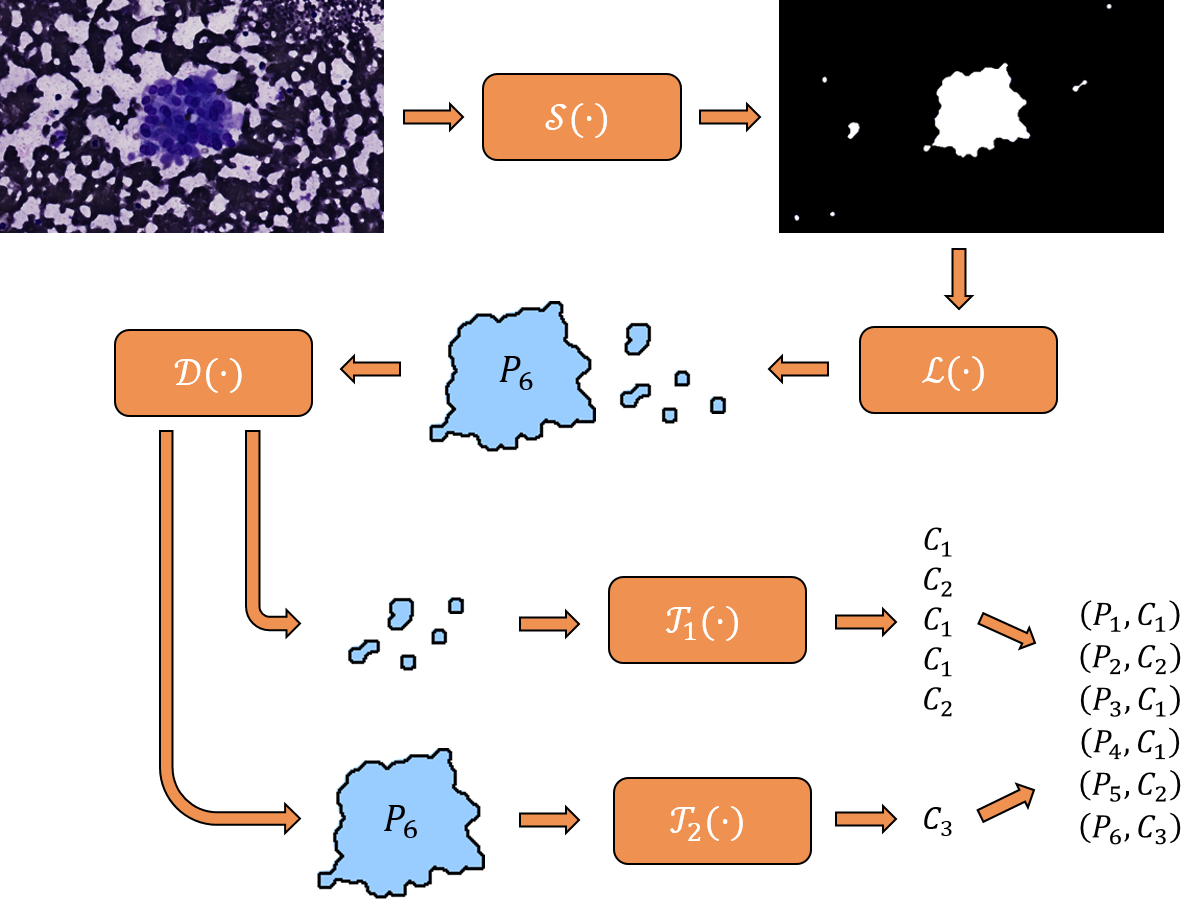
\includegraphics[scale=0.75]{image/workflow_illustration.png}
	\caption{Illustration of Algorithm \ref{algo:single_seg_several_classif}.}
	\label{fig:workflow_illustration}
\end{figure} 

Even though the workflow can now handle several types of objects, there are still some particular problems that cannot be solved with Algorithm \ref{algo:single_seg_several_classif}. In particular, this algorithm works perfectly as long as objects are not included in one another. In this case, the workflow will consider their intersection as a single object and therefore won't be able distinguish them.

Before extending the algorithm for handling this case, it is worth noting that Algorithm \ref{algo:single_seg_several_classif} is completely compatible with Algorithm \ref{algo:single_seg_single_classif}. Indeed, if there is only one classifier (i.e. $M = 1$) and the predicate $p_1$ always returns $true$, then both algorithms are exactly the same. 

\begin{algorithm}\label{algo:single_seg_several_classif}
Construction of the $\mathcal{W}$ operator with a single segmentation and several classifiers. 
\begin{enumerate}
	\item Apply the $\mathcal{S} \circ \mathcal{L}$ composition to the input image $\mathcal{I}$ to extract the objects of interest as the set of polygons $S_p \leftarrow \left\{P_1, ..., P_N \right\}$
	\item Initialize the labels set $L \leftarrow \emptyset$
	\item For each polygon $P \in S_p$:
	\begin{enumerate}
		\item Compute the classification label $C \leftarrow \mathcal{T}_{\mathcal{D}(P)}(P)$
		\item Place the label in the labels set $L \leftarrow L \cup \{C\}$
	\end{enumerate}
	\item Build and return objects and labels set $S_p \times L$.
\end{enumerate}
\end{algorithm}

\subsection{Chaining workflows}

To handle the case when some objects are included in others, a solution consists in executing several instances of Algorithm \ref{algo:single_seg_several_classif} one after another. 

\begin{definition}\label{def:several_w_op}
	Let $\mathcal{W}_1, ..., \mathcal{W}_K$ be a set of $K$ instances of Algorithm \ref{algo:single_seg_several_classif}. Each algorithm $\mathcal{W}_i$ has its own segmentation procedure $\mathcal{S}_i$ and proper sets of dispatching predicates $\mathcal{P}_i$ and classifiers $S_{\mathcal{T},i}$.
\end{definition}

While $\mathcal{W}_1$ would be applied to the full image $\mathcal{I}$ to extract all the objects of interest, $\mathcal{W}_2, ..., \mathcal{W}_K$ would only be passed image windows containing the previously detected objects. Given those windows, they would have to detect the objects of interest included in the objects found by $\mathcal{W}_1$. 

\begin{definition}\label{def:image_window}
	Let $\mathcal{I}_P \in I$ be an image window extracted from image $\mathcal{I}$ and containing the object represented by polygon $P$. The window is the minimum bounding box containing this polygon.
\end{definition}

A further refinement would be to provide a way for the implementer to filter the polygons of which the windows are passed to a given workflow instance. Indeed, a given instance $\mathcal{W}_i$ might be designed to process only a certain category of objects and therefore should not be passed windows of objects that doesn't fall in this category. 

\begin{definition}\label{def:filter_op}
	Let $\mathcal{F}$ be the $\textbf{filter}$ operator. It is given a set of polygons $S_P$ and returns a subset $S'_P$ of polygons:
	
	\begin{equation}
		\mathcal{F}(\cdot): H^N \rightarrow H^M, N, M \in \mathbb{N}, M \geq N
	\end{equation}
\end{definition}

Each instance of the workflow $\mathcal{W}_i$ except $\mathcal{W}_1$ is therefore associated a filter operator $\mathcal{F}_i$. The resulting algorithm is given in Algorithm \ref{algo:chaining_workflows} and has now reached an acceptable level of genericity. The algorithm is illustrated in Figure \ref{fig:chaining_illustration}.

\begin{algorithm} \label{algo:chaining_workflows}
	Construction of the $\mathcal{W}$ operator with $K$ instances of Algorithm \ref{algo:single_seg_several_classif}:

	\begin{enumerate}
		\item Execute the first workflow and save the results in the result set $R$: $R \leftarrow \mathcal{W}_1(\mathcal{I})$
		\item Create the polygons set and initializes it with the polygons found from the execution of $\mathcal{W}_1$: $S_P \leftarrow \left\{P_{1,1}, ..., P_{1,N}\right\}$
		\item For each $i \in \{2, ..., K\}$:
		\begin{enumerate}
			\item Extract polygons to be processed by $\mathcal{W}_i$: $S'_P \leftarrow \mathcal{F}_i(S_P)$
			\item For each polygon $P \in S'_P$:
			\begin{enumerate}
				\item Execute workflow $\mathcal{W}_i$ on the image window and saves the results: $R \leftarrow R \cup \mathcal{W}_i(\mathcal{I}_P)$
				\item Add the extracted polygons to the polygons set: $S_P \leftarrow S_P \cup \left\{P_{i,1}, ..., P_{i,M_i}\right\}$
			\end{enumerate}
		\end{enumerate}
		\item Return the results set $R$
	\end{enumerate}
\end{algorithm}

\begin{figure}
	\center
	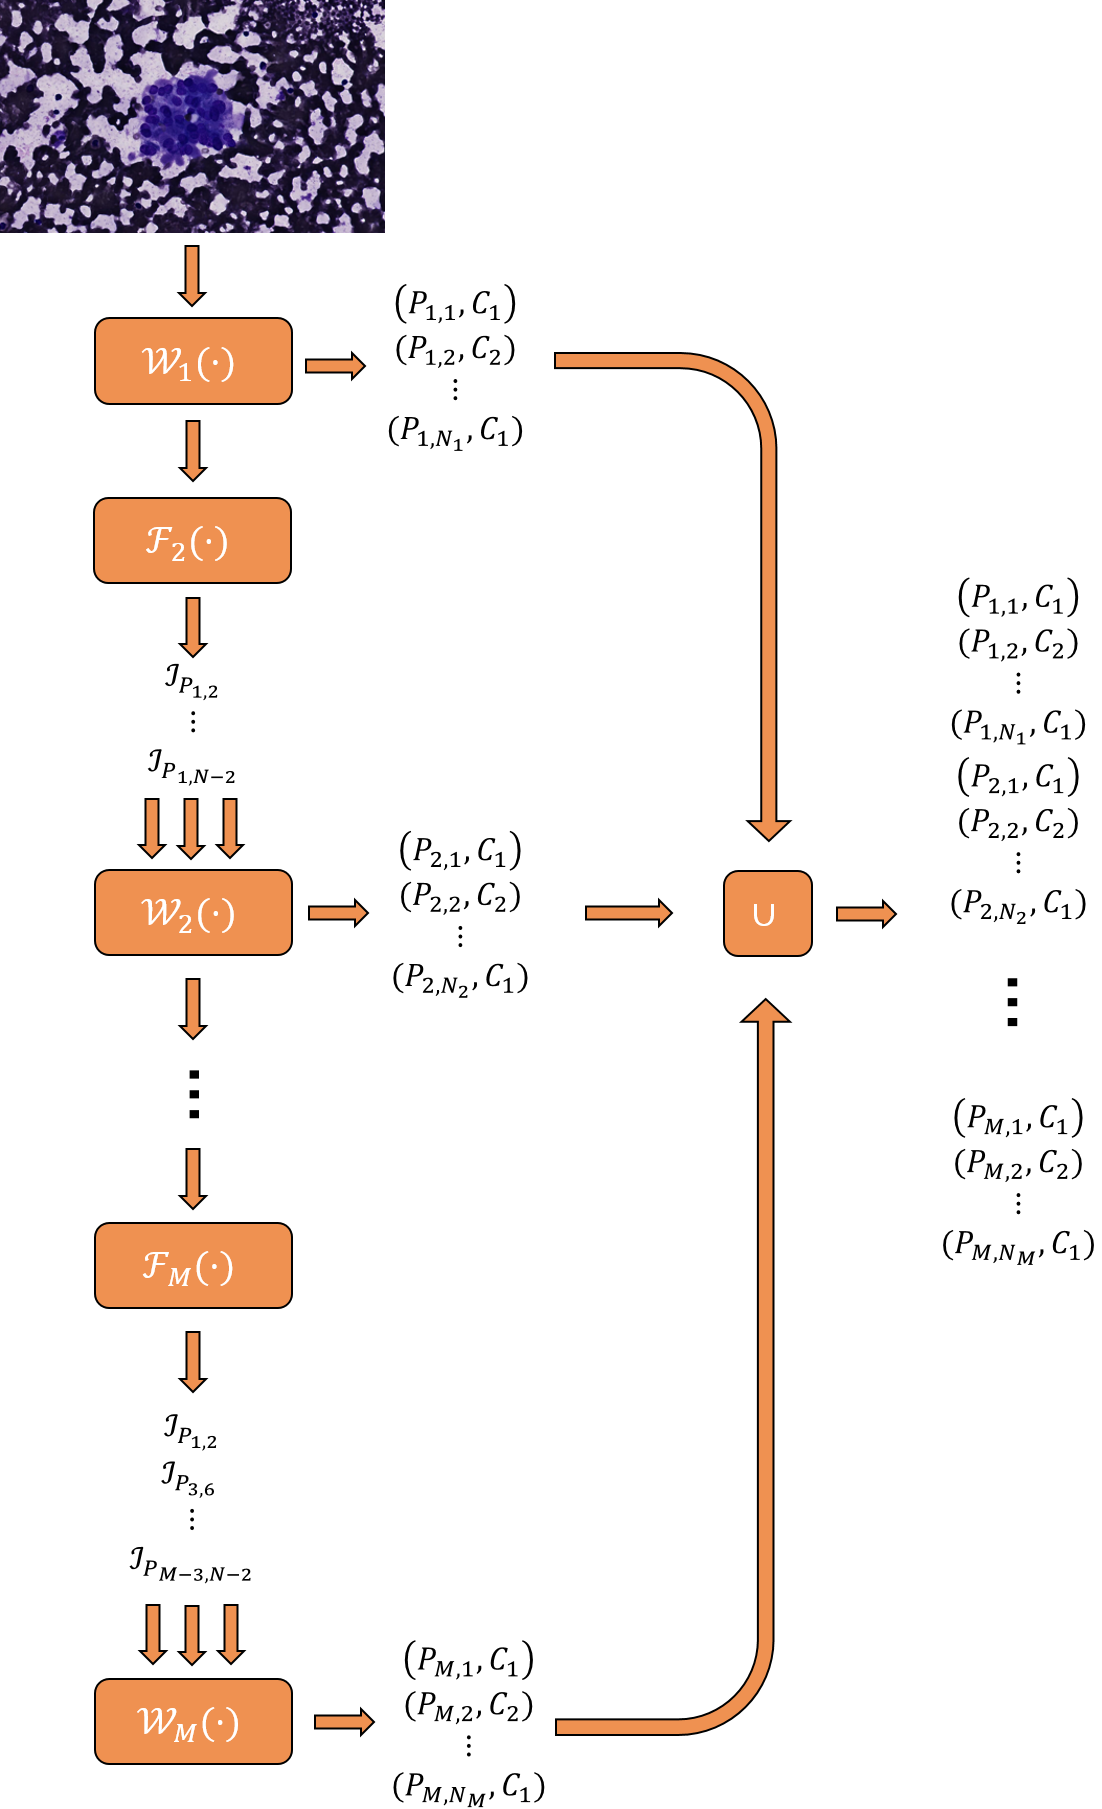
\includegraphics[scale=0.75]{image/chaining_illustration.png}
	\caption{Illustration of Algorithm \ref{algo:chaining_workflows}}
	\label{fig:chaining_illustration}
\end{figure}
\section{Implementation}
\label{sec:workflow_impl}
This section aims at presenting the implementation of the workflow formalized in Section \ref{sec:workflow_principle}. In Section \ref{ssec:work_init_impl}, the reasons why the previous implementation was replaced by a new one are presented. Then, the requirements, design choices and architecture of the new framework\footnote{In this section, the term \textit{workflow} will refer to the algorithm while \textit{framework} will refer to the implementation.} are given in Sections \ref{ssec:work_requirements}, \ref{ssec:work_language} and \ref{ssec:work_arch}. Finally, how to apply the framework is illustrated with a toy example in Section \ref{ssec:work_toy_example}. The framework discussed in this section is available on GitHub ?? at \href{https://github.com/waliens/sldc}{this url} ??.

\subsection{Initial implementation}
\label{ssec:work_init_impl}
As explained in this chapter's introduction, a first version of the workflow was implemented in 2015. However, in the context of this thesis, the decision was made to re-implement it for various reasons.

A major issue was the presence of a software component called a \textit{datastore} which had to be defined by the implementer for each distinct application of the workflow. In addition to be a dependency of almost every other class of the framework, it actually forced the implementer to define workflow execution and chaining logic himself although this logic is obviously not problem dependent and could be encapsulated. The major consequence of this design was an increased workload for the implementer to apply the framework to a custom object detection and classification problem. Moreover, the datastore being tightly coupled with other classes, it made writing automated tests quite difficult. Reproducing bugs was even harder because the replication implied to restore the datastore state which was not trivial. 

Another issue with the previous implementation was its too high level of genericity. Most of the components of the framework were defined as abstract classes and interfaces to be derived or implemented by the implementer. This made the framework hardly understandable and difficult to apply as he had to define more than just problem dependent components. In some cases, some implementations were provided but they only increased the complexity of the framework. Indeed, it was not clear whether those classes could be used directly or whether the implementer should provide his own classes.

Another final critical point was the lack of robustness. Especially, when applied to the thyroid case where images were fetched using HTTP requests, any network error would exit the program, leading to the loss of all collected data.

All in all, it was decided to re-implement the framework to get rid of the flawed parts of the design while keeping the good parts. The philosophy behind the new framework is illustrated through a set of requirements in Section \ref{ssec:work_requirements}.

\subsection{Requirements}
\label{ssec:work_requirements}
The main requirements for the framework are listed hereafter.

\paragraph{Genericity} As for the algorithm, the framework should be able to solve the widest possible range of object detection and classification problems in any context. This property has more implication in the case of the framework design than for the algorithm design, especially when it comes to fixing the representation of the various involved data types (i.e. image, polygon,...).

\paragraph{Efficiency} While the framework has no control over the efficiency of the algorithms defined by the implementer (i.e. segmentation or classification procedures), the coordination of those algorithms should not induce a significant overhead in the overall execution. 

\paragraph{Large images} While large images handling was irrelevant at the algorithm design stage, it becomes critical at this point. To remain generic, the framework should not make any assumption about the size of the images to be processed. Especially, a whole image should not be assumed to fit into memory.

\paragraph{Robustness} The framework should be robust to errors. That is, a single error should not interrupt the whole execution. For instance, if the framework executes a set of independent computations and one of them fails, it should only be stopped if this failure is unrecoverable and affects all the other computations. Otherwise, the failure should be reported and those others computations should execute until completion. 

\paragraph{Transparency} The framework should provide a built-in way to communicate its progress, the duration of each step as well as the errors it encounters with the user. The level of verbosity of this communication tool should be adjustable. Moreover, all the relevant information generated by the framework should be made available to the implementer in a structured and convenient way.

\paragraph{Parallelism} Whenever possible the framework should take advantage of parallelism to reduce its execution time but the implementer should be given a way to switch to sequential execution. Moreover, the implementer should be able to adjust the level of parallelism (i.e. the number of available processors).

\paragraph{Ease of use} The work of the implementer should be kept as minimal as possible. He should only have to define the logic of the workflow components that are problem dependent : image format, segmentation, dispatching rules, classifiers,... 

\subsection{Language}
\label{ssec:work_language}
The first choice occurring in the development of an existing algorithm is obviously the language in which it will be implemented. As far as the workflow is concerned, the chosen language was Python. Indeed, this language provides a simple, accessible and complete environment for solving the kind of problems addressed by the framework and would therefore contribute to the overall ease of use the framework. 

First of all, the language has many features which allows developers to quickly come up with solutions to problems. Especially, it is strongly and dynamically typed, multi-paradigm (imperative, functional, object oriented,...), interactive (it can be used in an interactive console), interpreted and garbage-collected. It also supports usual data structures such as lists, arrays, dictionaries and sets natively and provides operations for manipulating them in a concise way. 

In addition to its built-in features, Python has become a great language for scientific computing as it has been augmented with excellent open source libraries over the years. First, the SciPy ecosystem which includes the SciPy \cite{oliphant:2007} and NumPy \cite{vanderwalt:2011} libraries. The first is a collection of numerical algorithms and domain-specific toolboxes (signal processing, optimization, statistics,...). The second is a fundamental package for numerical computations which provides an efficient representation of multi-dimensional arrays and operations on them. Built on top of the SciPy ecosystem comes Scikit-Learn \cite{pedregosa:2011}, a library that provides simple, efficient and reusable tools for data mining and machine learning. Image processing is not outdone with a Python binding for the huge OpenCV library \cite{opencv_library}. Two alternatives are scikit-image \cite{scikit-image} which is built on top of the SciPy ecosystem or the Pillow library \cite{pillow}. All of them provide a collection of well-known image processing algorithms. Another useful library is Shapely \cite{shapely} which provides a representation for geometrical objects (e.g. polygons) and operations on them. 

Python was also chosen because the workflow was implemented to be integrated with Cytomine (see Section ??). Particularly, the final goal was the detection and classification of objects in images stored on Cytomine servers. As those images and their metadata are exposed through an API interfaced by a Python client, it was essential that the workflow could use this client to communicate with the back-end. As the Cytomine client was implemented in the version 2.7.11 of Python, this version was also used for developing the framework. 

\subsection{Software architecture}
\label{ssec:work_arch}
The framework was organized as a Python library of which the root package was called \texttt{sldc}. 

\subsubsection{Image representation} 
\label{sssec:work_image_repr}
The image representation design is a critical point of the framework architecture. Indeed, on the one hand, it should be abstract enough so that implementers can apply the workflow on images in any format. On the other hand, it should provide access to a concrete representation available to the framework because some steps need to access this representation to extract some information. For instance, location is one such step as it processes a binary mask to extract polygons. 

The representation should also provide a way of extracting sub-windows from an image. The need for this feature is twofold. First, it is needed by the workflow (see Definition \ref{def:image_window}). Then, it could be used to address the large images handling requirement and to overcome the fact that a whole image is not assumed to fit into memory. The idea is to split the image into smaller chunks called tiles which could be loaded into memory and processed one after another. Especially, the tiles would be applied the first part of the workflow, that is segmentation and location. As the polygons of each tile are extracted independently, it might occur that a single object of interest which spreads over several tiles ends up being splitted into several polygons. To make sure there is a one to one relationship between a polygon and an object of interest, an additional step must be added to the workflow before the dispatching and would consist in merging the polygons representing a same object. This step is detailed in Section \ref{sssec:merging}.

The abstract image representation and related classes were implemented into the \texttt{sldc.image} package presented in the UML diagram shown in Figure \ref{fig:uml_image_package}.

The \texttt{Image} class is the abstract image representation mentioned above. It provides three abstract methods for checking image dimensions (width, height and number of channels) and a fourth one, \texttt{np\_image}, which should implement the conversion between the implementer's custom image format and the concrete format mentioned above. NumPy multi-dimensional arrays were chosen to be this concrete representation. In addition to the inherent advantage of using the NumPy library, this choice was also motivated by the fact that those arrays are compatible with the various image processing libraries presented in Section \ref{ssec:work_language}. 

An image window is materialized by the \texttt{ImageWindow} class of which the design is based on the decorator pattern. It stores information about the position and size of the window as well as a reference to the parent image. Especially, location and size are respectively represented by coordinates of the first top left pixel included in the window (coordinates are referenced to the top left corner of the parent image) and by the window width and height. As an image window instance provides a level of indirection on top of another image, some methods are provided to fetch this base image as well as the absolute offset\footnote{The absolute offset is the offset of the window referenced to the base image's top left pixel. It is different from the image window offset if its parent image is also an image window.}.

A tile is also represented by a class named \texttt{Tile} which extends \texttt{ImageWindow} and augment it with an integer identifier field. As tiles can potentially be derived, a \texttt{TileBuilder} interface was developed. As suggested by the name, a class implementing this interface is responsible for building specific tile objects. This structure is actually an application of the factory method pattern which has the advantage of allowing the framework to build specific tiles objects defined by the implementer while remaining unaware of the construction logic of those objects. The implementer that would derive the \texttt{Tile} class to implement a custom loading procedure in \texttt{np\_image} is advised in the documentation to raise an \texttt{TileExtractionError} exception if the loading fails. This allows the rest of the framework to handle loading failure and therefore increase its robustness. 

Finally, to make it easier to iterate over the tiles of an image two classes were developed : \texttt{TileTopology} and \texttt{TileTopologyIterator}. The first is responsible for dividing an image into a set of overlapping tiles. The overlap allows the merging procedure to be simpler as polygons corresponding to a same object will have a geometrical intersection. 

The tile topology is fully defined with three parameters: the tile maximum width, $w_m$, and height, $h_m$, and the number of pixels that overlap, $o_p$. The tile topology object also associates unique increasing identifiers to the tiles. An example topology with its resulting tiles and identifiers is shown in Figure \ref{fig:tile_topo_example}. As soon as the \texttt{TileTopology} object is built, it can be queried using those identifiers for building tile objects or for fetching topology information such as one tile's neighbours identifiers. While this organization goes off from the object oriented philosophy a bit, it allows all operations provided by the tile topology object to be $\mathcal{O}(1)$ (see Appendix \ref{apdx:tile_topology}). It goes without saying that the overlap parameter should be set carefully because it induces some additional computations. Indeed, some parts of the image will be segmented several times as they are present on more than one tile. 

The second class, \texttt{TileTopologyIterator}, is an application of the iterator design pattern as its name suggests. It can be created either from a tile topology or directly from a subclass of \texttt{Image}. It allows to iterate over the tiles defined by a tile topology. The implementation of this iterator is straightforward. It simply iterates over the tile identifiers and pass them to the corresponding tile topology to build the tiles. 

\begin{figure}[h]
	\center 
	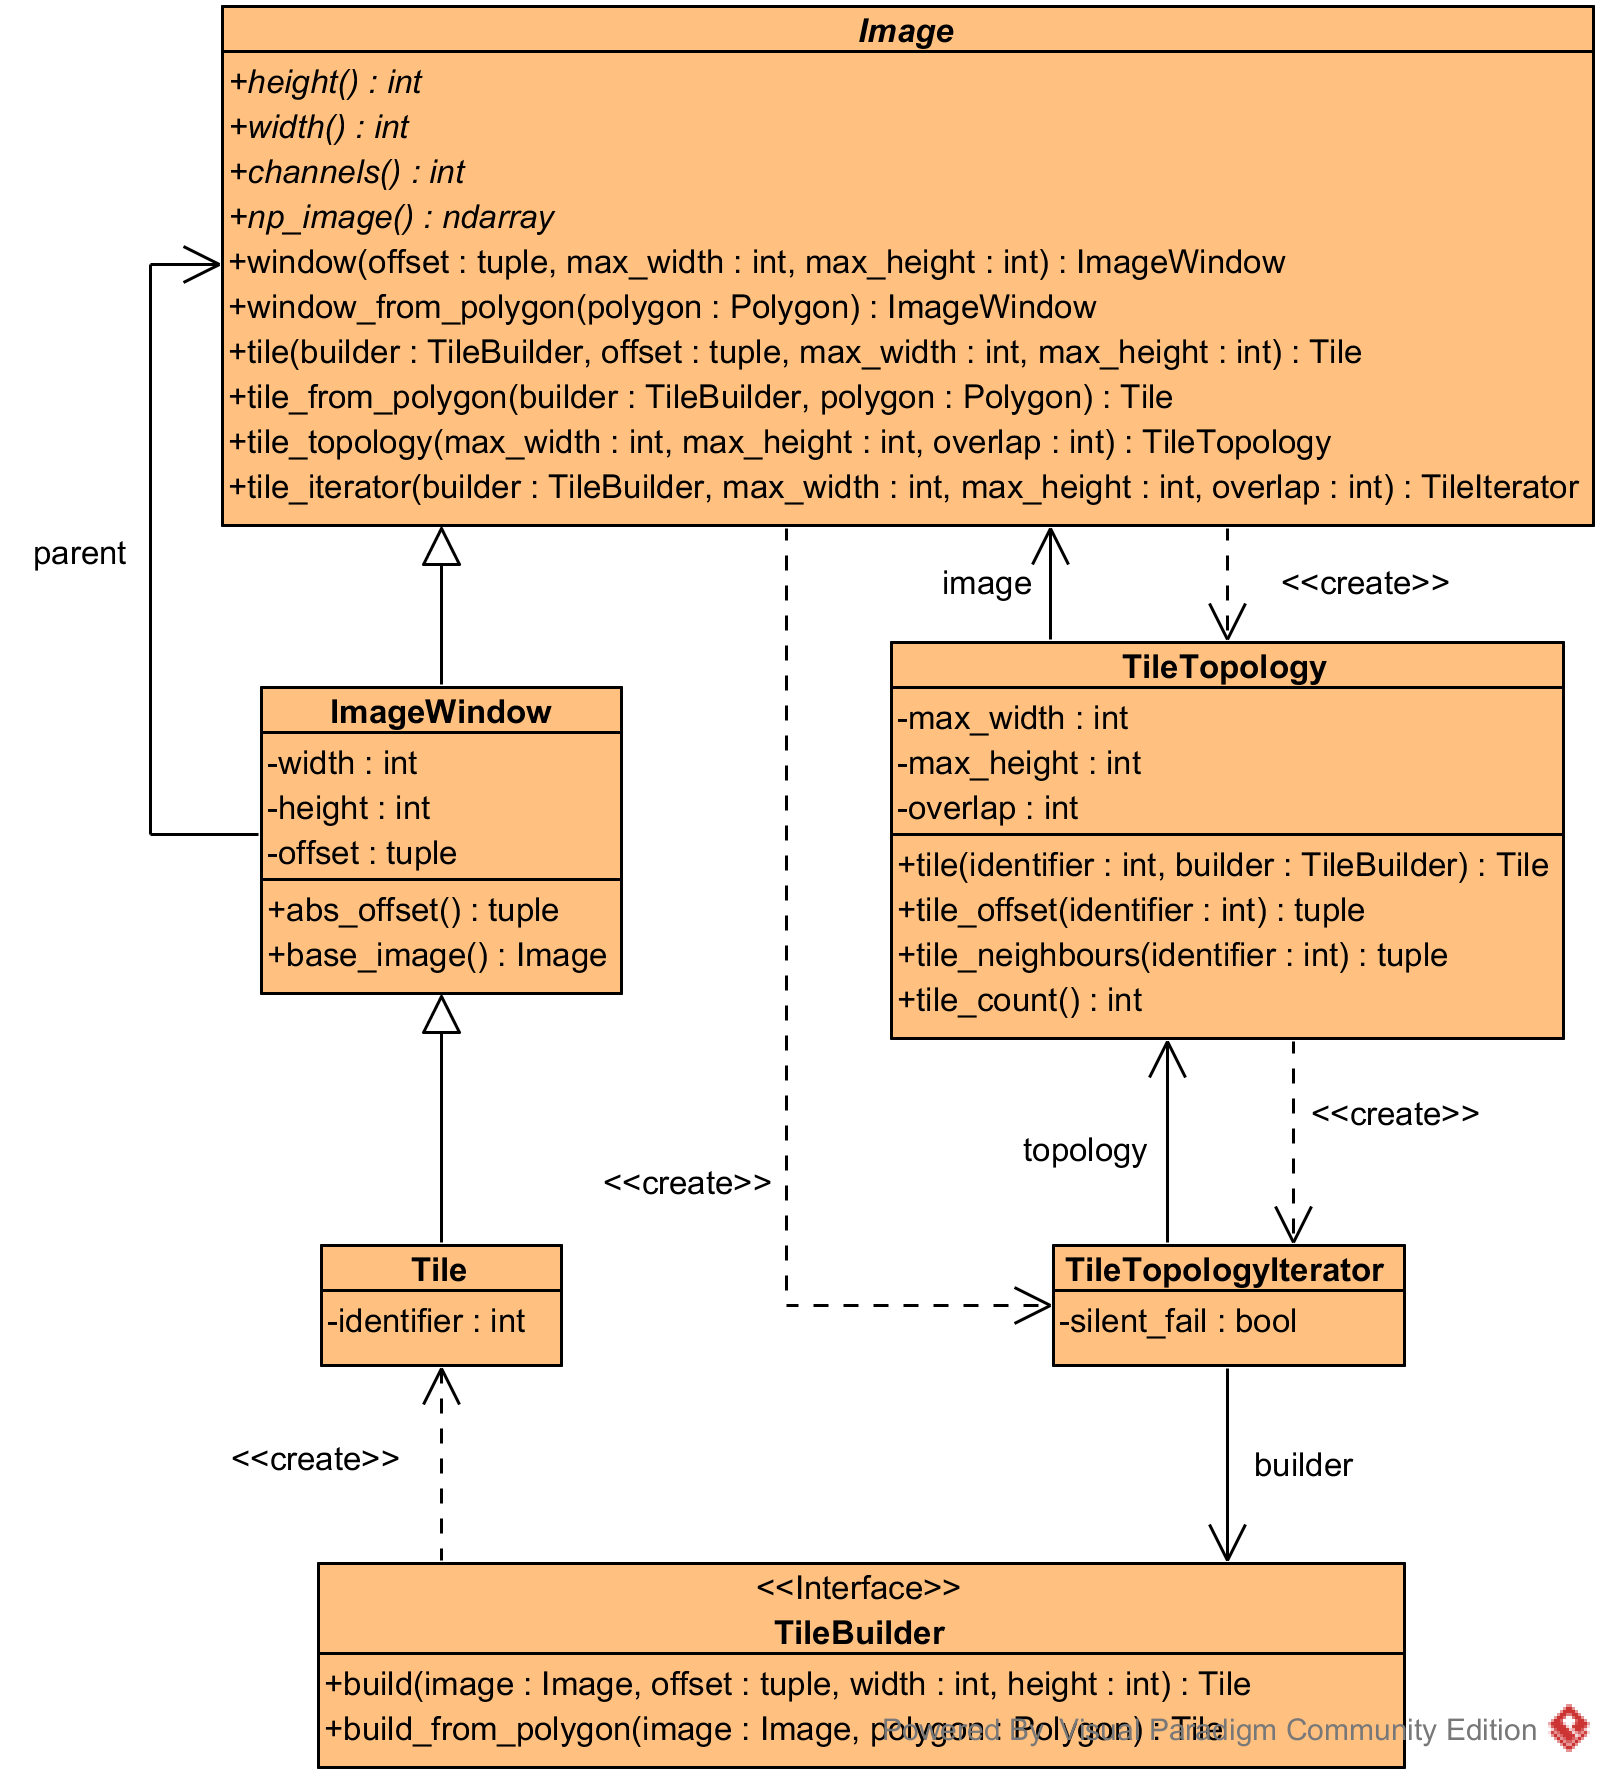
\includegraphics[scale=0.9]{image/uml_image_package.png}
	\caption{Image representation classes - package \texttt{sldc.image}}
	\label{fig:uml_image_package}
\end{figure}

\begin{figure}[h]
	\center
	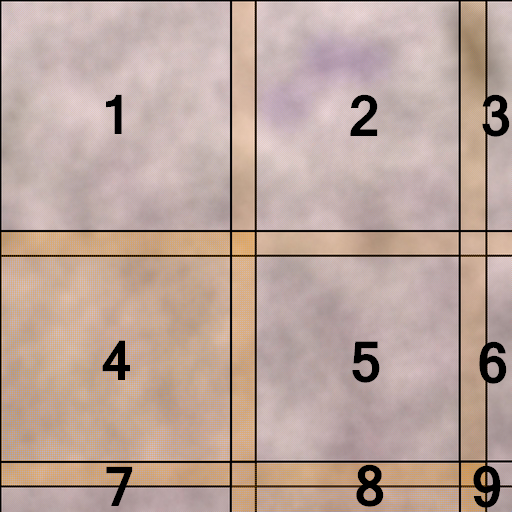
\includegraphics[scale=0.5]{image/tile_topo_2048_2048.png}
	\caption{A tile topology applied on a $512\times 512$ image (parameters: $w_m = 256$, $h_m = 256$ and $o_p = 25$). The numbers are the tile identifiers.}
	\label{fig:tile_topo_example}
\end{figure}

\subsubsection{Segmentation}
As explained in Section \ref{ssec:single_single}, the segmentation is not fixed by the framework and the implementer is expected to provide its own implementation. To represent this constraint in the framework, a \texttt{Segmenter} interface was defined in package \texttt{sldc.segmenter}. It provides a single method, \texttt{segment}, which receives a NumPy representation of the image and is expected to return another NumPy array storing the binary mask marking the objects of interest contained in this image. The binary mask however doesn't conform strictly to Definition \ref{def:segmentation_op} as pixels belonging to an object of interest are marked with the integer value 255 (which corresponds to white in the grayscale color space) instead of 1. The \texttt{Segmenter} interface is Shown in Figure \ref{fig:uml_pack_seg_merg_loc_classif}.

\begin{figure}
	\center 
	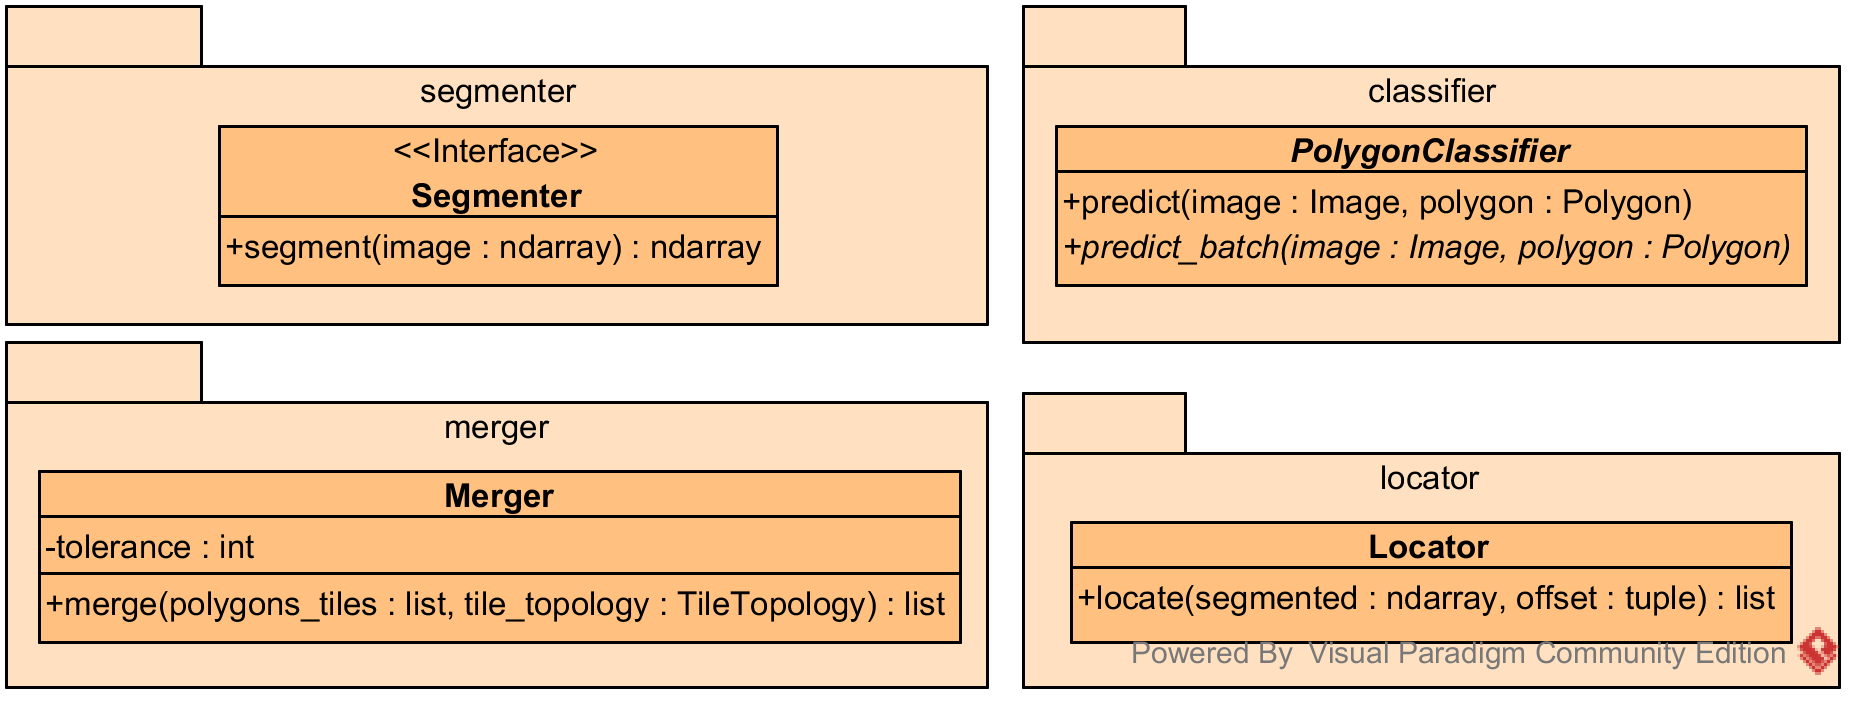
\includegraphics[scale=0.95]{image/uml_seg_merg_loc_classif.png}
	\caption{Packages \texttt{sldc.segmenter}, \texttt{sldc.locator}, \texttt{sldc.merger} and \texttt{sldc.classifier}.}
	\label{fig:uml_pack_seg_merg_loc_classif}
\end{figure}

\subsubsection{Location}
As presented in Definition \ref{def:locate_op}, the location procedure extracts polygons representing the geometrical contours of the objects of interest from a binary mask. The implementation of this operation was done in the single method, \texttt{locate}, of a class called \texttt{Locator} (in package \texttt{sldc.locator}). This method takes as parameter the binary mask represented by a NumPy array and returns the expected set of polygons as Shapely \texttt{Polygon} objects.
 
As stated in Section \ref{ssec:single_single}, this operation can be fixed by the framework without loss of genericity. This is made possible by the choice of representation for the method's inputs and outputs. As far as the implementation is concerned, it was largely inspired from another implementation taken from the Cytomine codebase. It uses the \texttt{findContours} procedure of the OpenCV library to extract the geometrical information of the objects as a list of coordinates. The implementation provided with the framework has two small additions compared to the Cytomine one. The first is the conversion of those coordinates into \texttt{Polygon} objects and the second is an optional translation that can be applied to those polygons. This second modification is needed because of the image division in tiles. Indeed, by default, the location algorithm constructs polygons referenced to the top-left pixel of the binary mask passed to \texttt{locate}. Yet, the polygons are expected to be referenced to the full image top-left pixel. An additional parameter was therefore added to the \texttt{locate} method prototype allowing the caller to specify a translation offset to apply to the found polygons. The \texttt{Locator} class is Shown in Figure \ref{fig:uml_pack_seg_merg_loc_classif}.

\subsubsection{Merging}
\label{sssec:merging}
The need for a merging phase is a consequence of the image division in tiles and its goal is to merge distinct polygons that actually represent a same object of interest. The main idea behind the algorithm was imagined by ?? JM Begon ??. It consists in building a graph where each node corresponds to a polygon. The algorithm will then add edges between polygons which correspond to a same object. Two polygons represent a same object if the distance between them (i.e. minimum distance between one point of each polygon) is less then a certain tolerance threshold. Generating the final polygons is as simple as finding all the connected components of this graph and computing the intersection of all the polygons in those components. 

While working in some cases, the implementation made by Jean-Michel Begon could be improved. First, the interface of the class was inconvenient to use. Indeed, the tiles and their polygons had to be provided in a fixed order (i.e. increasing order of identifiers). And if they weren't, the merging would fail. Moreover, it had issues with some border cases. For instance, with small images containing few tiles. For those reasons, the algorithm was kept but was completely reimplemented to take advantage of the \texttt{TileTopology} object (which didn't exist in the previous implementation of the workflow). 

The classes related to merging were defined in the package \texttt{sldc.merger}. The main logic of the algorithm was implemented in a class called \texttt{Merger}. Applying a merge is as simple as passing a tile topology as well a the tiles and associated polygons to the \texttt{merge} method which return the list of merged polygons. The \texttt{Merger} class is Shown in Figure \ref{fig:uml_pack_seg_merg_loc_classif}.

\subsubsection{Dispatching and classification}
\label{sssec:dispatch}
As defined in Section \ref{ssec:single_several}, the dispatching of polygons to classifiers is performed using predicates. Those predicates are materialized by the abstract class \texttt{DispatchingRule} in package \texttt{sldc.dispatcher}. The implementer can extend to define its custom dispatching logic. Especially, this is done by implementing the method \texttt{evaluate\_batch} which is passed both a list of polygons to dispatch as well as the image from which they were extracted. Passing both the polygons and the image allows the implementer to define a dispatching logic based on either the polygons geometrical properties, or the polygons crops, or both.  

The same philosophy was followed for classification. The implementer has to extend the abstract class \texttt{PolygonClassifier} from package \texttt{sldc.classifier} (see Figure \ref{fig:uml_pack_seg_merg_loc_classif}). For the same reason as for the \texttt{evaluate\_batch} method, the \texttt{predict\_batch} methods takes as parameters a set of polygons and the image they were extracted from. Although only a label is produced by the classifier operator in Definition \ref{def:classif_op}, an additional element is returned by the \texttt{predict\_batch} method: the class probability (i.e. the probability that the predicted label is indeed the label of the object). Indeed, this information can sometimes be extracted using some classifiers (e.g. tree based methods). However, it can happen that the underlying classifier is not able to generate those probabilities. In this case, the implementer is advised to return a probability 1 for each polygon. The class \texttt{PolygonClassifier} is shown in Figure \ref{fig:uml_pack_seg_merg_loc_classif}.

While the dispatching and classification logic are problem dependent, the coordination of those steps is obviously not and is implemented in class \texttt{DispatcherClassifier} (see Figure \ref{fig:uml_dispatcher_classifier}). This object must be initialized with a set of classifiers and dispatching rules. Some polygons can then be dispatched and classified by passing them to the methods \texttt{dispatch\_classify} or \texttt{dispatch\_classify\_batch}. Especially, the first will execute the operation on a single polygon while the second allows to process a set of polygons. 

To answer the transparency requirement, it is essential that all the relevant information generated by these methods can be accessed by the implementer after the execution. Those information obviously include the classification label and its associated probability but not only. Indeed, another relevant information generated is the identity of the dispatching rule which matched a polygon. In practice, this information can be used by the implementer to distinguish a same classification label returned by different classifiers. The \texttt{dispatch\_classify} method therefore returns a tuple containing the label, the probability and the identifier of the dispatching rule that matched the polygon (this identifier being the index of the rule in the list passed at construction). The \texttt{dispatch\_classify\_batch} method  returns three lists containing the same information for all the passed polygons.
\paragraph{}
In the workflow, it is assumed that one and only one dispatching predicate can be true at once. In practice, the framework should handle sets of predicates which don't verify this property. Especially, it should handle a first case when more than one rule match a polygon and a second case when no rule matches a polygon. 

The first case is handled by ordering the rules and to only consider the first rule that matched. Especially, the ordering is defined by the order of the rules in the list provided by the implementer at construction. 

The second case is handled with a fail callback. This function is passed the polygon that didn't match any rule and return a value or object that will be used as classification label. A default callback which always returns \texttt{None}\footnote{\texttt{None} is the \texttt{null} equivalent of Python.} is used if the implementer doesn't provide one.
Moreover, the dispatch index associated to those unmatched polygons is -1.


\begin{figure}
	\center
	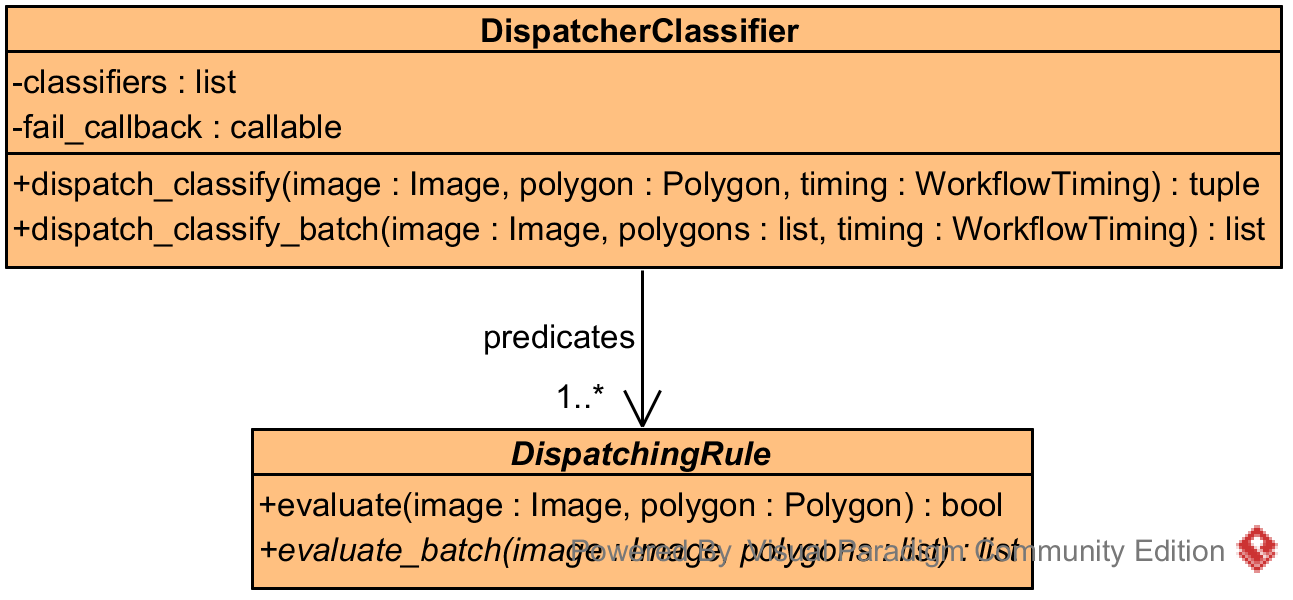
\includegraphics[scale=0.95]{image/uml_dispatcher_classifier.png}
	\caption{Package \texttt{sldc.dispatcher}}
	\label{fig:uml_dispatcher_classifier}
\end{figure}

\subsubsection{Workflow}

The package \texttt{sldc.workflow} contains the actual implementation of Algorithm \ref{algo:single_seg_several_classif}, in \texttt{SLDCWorkflow} class. Instantiating this class requires three mandatory parameters: a \texttt{Segmenter} which implements the tile segmentation logic, a \texttt{DispatcherClassifier} which was initialized with custom dispatching rules and polygon classifiers and a \texttt{TileBuilder} for building the tiles of the tile topology. The workflow can then be launched on an \texttt{Image} object using the method \texttt{execute}. This method returns all the information about the objects of interest found in the image. Those information include the polygons encoding the object's shapes and locations, their predicted classes, the associated probabilities and the dispatching indexes (see Section \ref{sssec:dispatch}). In order to provide a convenient access to those information, they were encapsulated into an object called \texttt{WorkflowInformation}. Especially, this class provides a way to iterate over the results, the method \texttt{results}. The UML diagram containing both the \texttt{SLDCWorkflow} and \texttt{WorkflowInformation} classes is given in \ref{fig:uml_workflow}.

\begin{figure}
	\center
	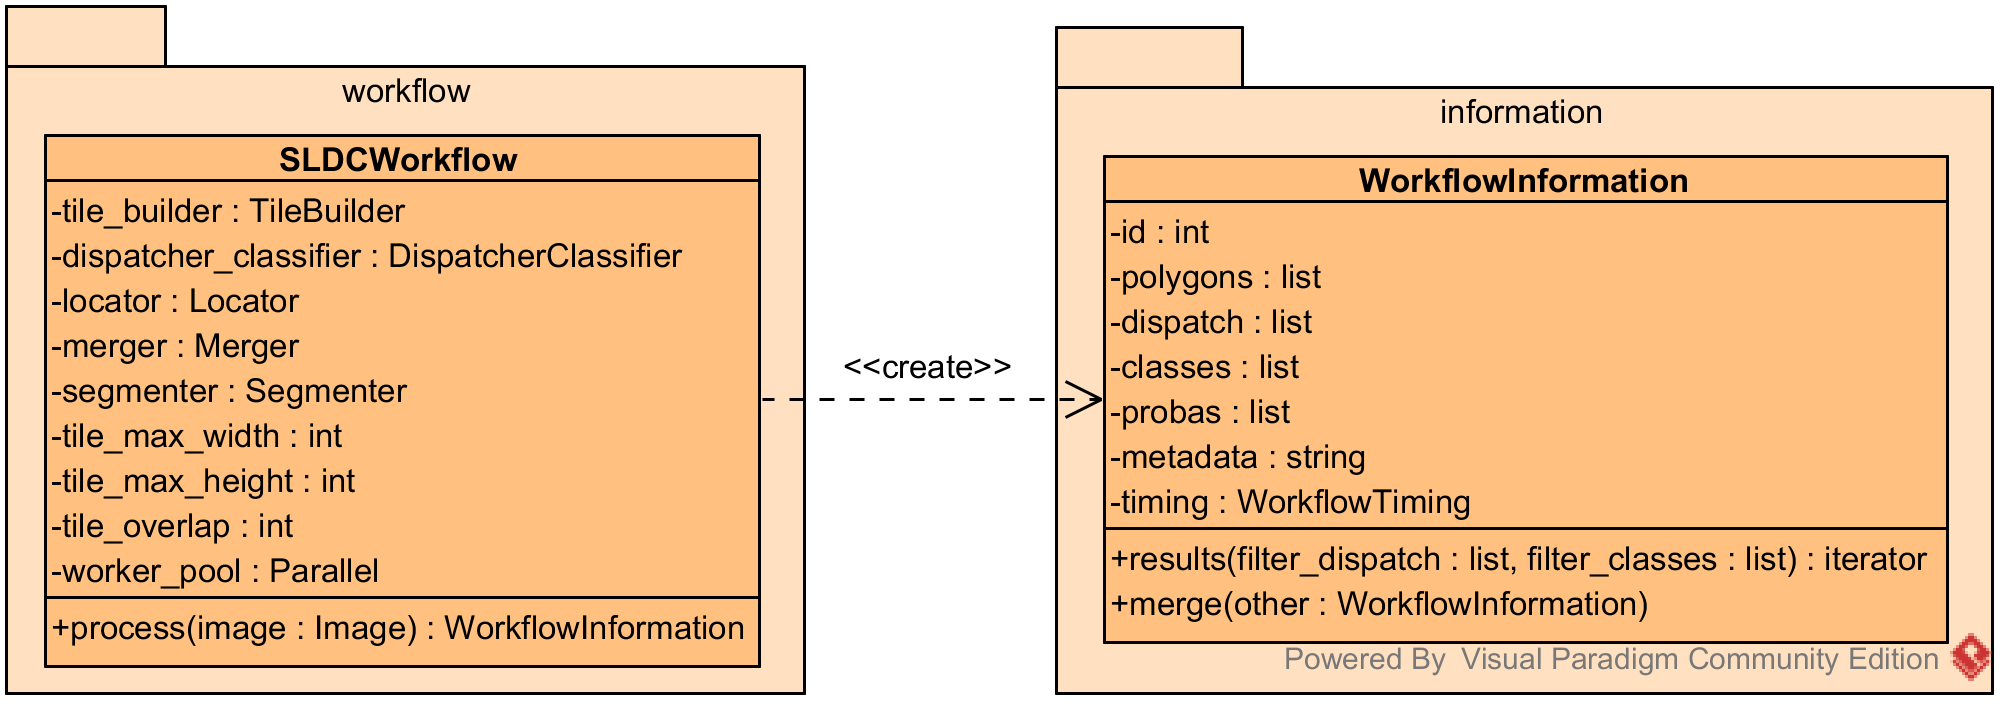
\includegraphics[scale=0.75]{image/uml_workflow.png}
	\caption{Package \texttt{sldc.workflow} and class \texttt{WorkflowInformation}}
	\label{fig:uml_workflow}
\end{figure}

\subsubsection{Workflow chain}
To this point, the presented classes provide a way for an implementer to apply Algorithm \ref{algo:single_seg_several_classif}. The package \texttt{sldc.chaining} allows to go one step further as it contains the necessary components for applying Algorithm \ref{algo:chaining_workflows}. Especially, the class \texttt{WorkflowChain} coordinates the execution of several workflows one after another on one or more images and also handles the post processing of the generated data. Those operations are handled by different components defined hereafter. The UML diagram containing the classes of this package is shown on Figure \ref{fig:uml_chaining}.

The images to be processed by the workflow must be generated by an implementation of the interface \texttt{ImageProvider}. The implementer must define the image generation in the abstract method \texttt{get\_images}. 

The post processing of the generated data must be defined by the implementer as \texttt{PostProcessor} object. Especially, he has to implement the method \texttt{post\_process} which is passed a collection of workflow information objects as well as the image from which they were generated.

As far as the workflow objects to be executed are concerned, they must be encapsulated into subclasses of \texttt{WorkflowExecutor}. This component has three main responsibilities. 

The first is to generate the image windows that will actually be processed by the underlying \texttt{SLDCWorkflow} object. Particularly, those windows must be generated based on the polygons generated from the previous steps of the chain. This generation must be implemented in the \texttt{get\_windows} method. This method is also the placeholder for the filtering specified in Definition \ref{def:filter_op}. As far as the first workflow of the chain is concerned, its \texttt{get\_windows} method should have a slightly different behavior. Indeed, in this case, the full image is yet to be processed and should be returned. In the optic to reduce the work of the implementer, a abstract subclass named \texttt{FullImageWorkflowExecutor} was defined to implement this behavior. Its \texttt{get\_windows} method simply returns the image it is passed. 

The second responsibility is to launch the \texttt{execute} method of the \texttt{SLDCWorkflow} object on the images generated by the executor in \texttt{get\_windows} and to collect the generated workflow information objects. This is done in the \texttt{execute} method. 

The last responsibility is the post-processing of the results generated by one workflow execution. This logic must be implemented in the method \texttt{after} which is passed the image window that was processed as well as the workflow information object returned by the \texttt{execute} method of \texttt{SLDCWorkflow}. An example usage of this method is the translation of polygons generated by a \texttt{SLDCWorkflow} on an image window. Indeed, in this case the polygons returned by the workflow object are reference to the window top left pixel while they should be referenced to the full image top left pixel. For the same reason as the \texttt{FullImageWorkflowExecutor}, a subclass of \texttt{WorkflowExecutor} was created. Its \texttt{after} method implements the translation logic.

As soon as the \texttt{ImageProvider}, \texttt{PostProcessor} and \texttt{WorkflowExecutor} objects are constructed, they should be passed to the \texttt{WorkflowChain} constructor. The chain can simply be started by calling the \texttt{execute} method.

\begin{figure}
	\center
	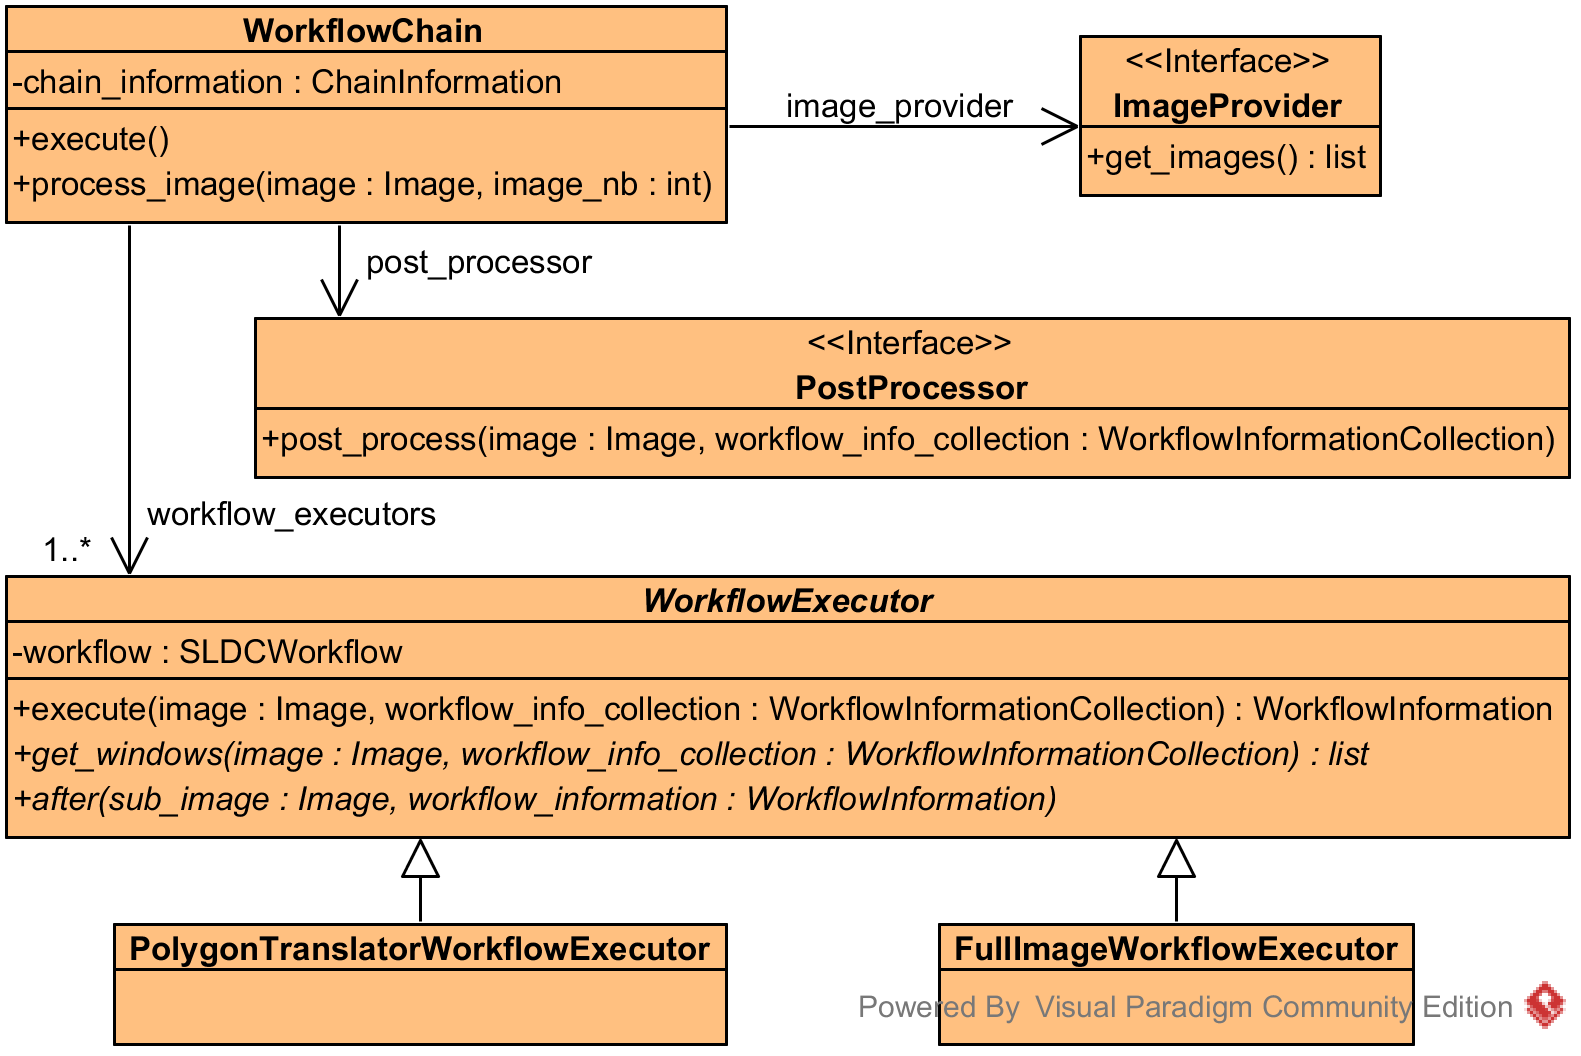
\includegraphics[scale=0.75]{image/uml_chaining.png}
	\caption{Package \texttt{sldc.chaining}}
	\label{fig:uml_chaining}
\end{figure}

\subsubsection{Logger and workflow timing}
To fulfill the transparency requirements, it is essential that the person who executes a workflow chain is able to monitor the progress. He should also have some insights about how the workflow performs on a given problem. For instance, how many tiles must be processed, how many polygons were found, how many polygons were dispatched,... The user should also be informed about the execution times of the various phases. In order to perform those operations two other packages were added. 

\paragraph{Logging} The first one is \texttt{sldc.logger} which provides a flexible, powerful and thread-safe logging system. Especially, it allows to log messages selecting a level verbosity among \textit{silent}, \textit{debug}, \textit{info}, \textit{warning} and \textit{error}. The output can be controlled using a minimum level of verbosity. All messages sent below this level won't be outputted. The implementer can also choose where the messages will be printed (in a file, on the standard output,...).

The logging package is articulated around the abstract class \texttt{Logger} which holds the minimum level of verbosity and provides methods to log messages in all the defined levels of verbosity. It also implements the message formatting. Especially, the messages sent by the implementer are augmented with a prefix containing the thread id, the current date and time as well as the level of verbosity at which it was sent. 

What this class doesn't define is where the formatted messages will be printed. This is the responsibility of the subclasses. Three of them are provided in the package: \texttt{StandardOutputLogger}, \texttt{FileLogger} and \texttt{SilentLogger}. The first one prints the messages into the program's standard output, the second prints them into a file while the last ignores all messages. If the implementer is not satisfied with one of those implementation, he can define himself a subclass that handle messages in a custom way. 

The final component of the package is an abstract class called \texttt{Loggable}. Its first goal is self documentation for the classes which extend it. Indeed, those are expected to support logging. The second goal is to provide a logger attribute for the classes which extend it. This way, they don't have to define their own. 

The UML diagram of the logging package is shown in Figure \ref{fig:uml_logging}.

\paragraph{Timing} The second package, \texttt{sldc.timing}, contains the \texttt{WorkflowTiming} class which allows to record execution times of the various phases of the workflow but also to report them. The time computation is provided through some \texttt{start} and \texttt{end} methods for each phase. For instance, for recording segmentation time, the methods \texttt{start\_segmentation} and \texttt{end\_segmentation} are provided. The phases that can be recorded are the following: image loading, segmentation, location, merging, dispatching and classification. A last phase is actually a combination of the loading, segmentation and location phases and is called \textit{lsl}. An additional method is needed for this combination because it can be parallelized (see Section \ref{sssec:work_parallel}). Recorded execution times can be extracted with a handful of methods such as \texttt{total} which computes the total recorded time for all phases, or \texttt{report} which is passed a \texttt{Logger} object and prints some statistics about the execution times. The UML diagram of this package is shown in Figure \ref{fig:uml_timing}.

\begin{figure}
	\center
	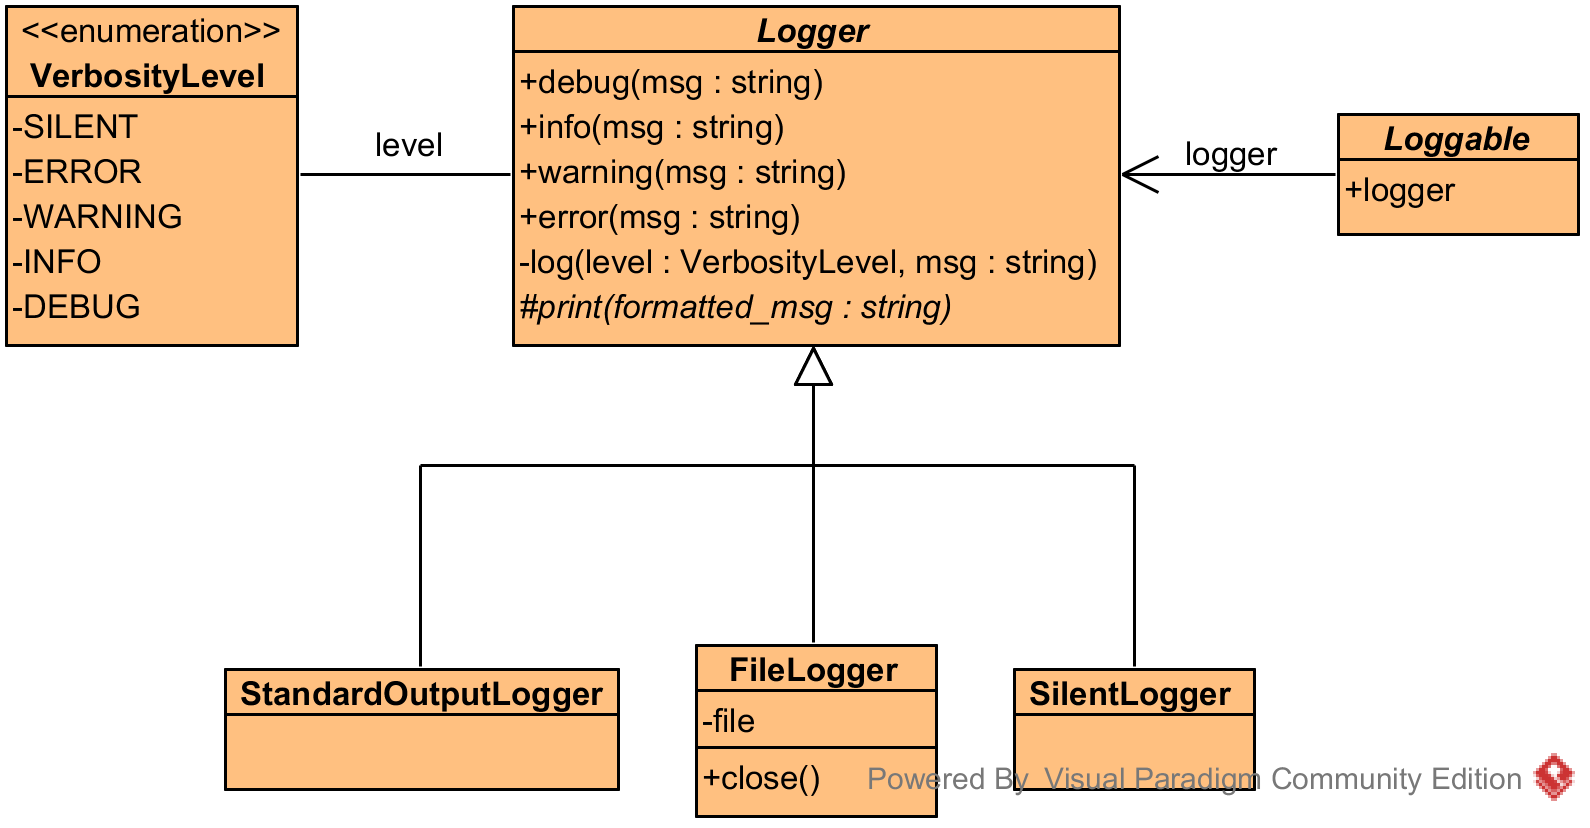
\includegraphics[scale=0.75]{image/uml_logging.png}
	\caption{Package \texttt{sldc.logging}.}
	\label{fig:uml_logging}
\end{figure}

\begin{figure}
	\center
	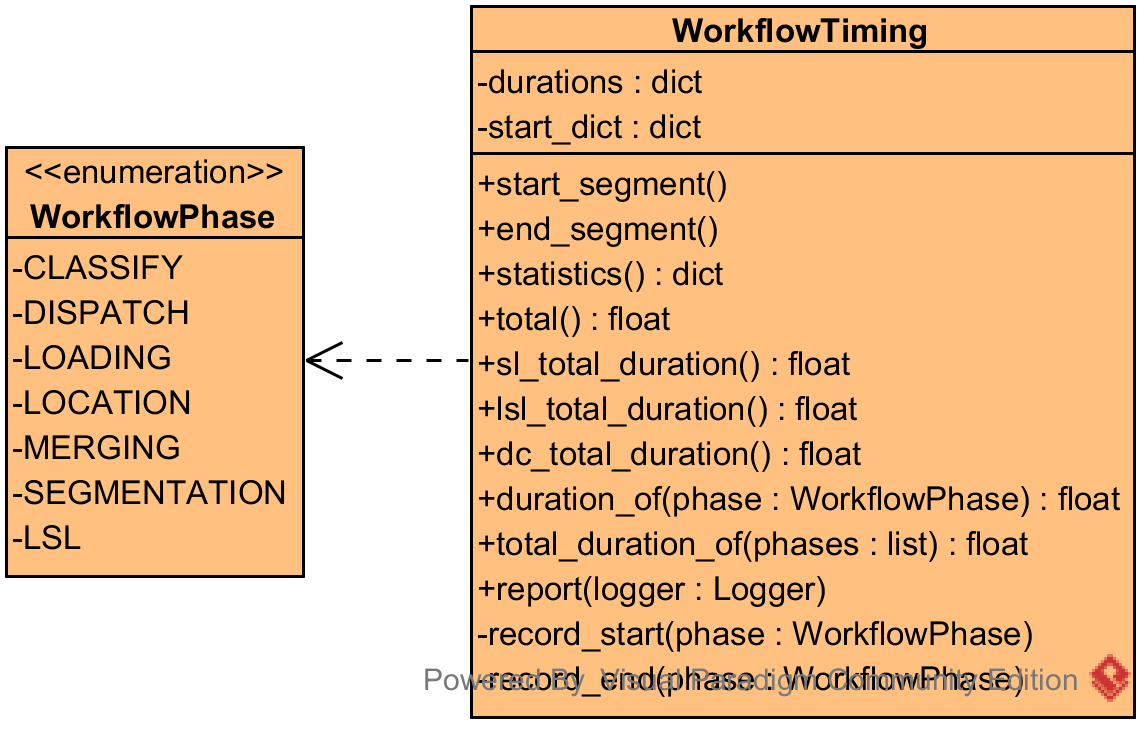
\includegraphics[scale=0.75]{image/uml_timing.png}
	\caption{Package \texttt{sldc.timing}.}
	\label{fig:uml_timing}
\end{figure}

\subsubsection{Builders}
The package \texttt{sldc.builder} contains two classes \texttt{WorkflowBuidlder} and \texttt{WorkflowChainBuilder} for making easier the construction of \texttt{SLDCWorkflow} and \texttt{WorkflowChain} objects respectively. Those classes provide some methods for setting the construction parameters and a \texttt{get} method for actually constructing the expected object based on the provided parameters. For instance, the \texttt{WorkflowBuilder} provides a method \texttt{set\_segmenter}. The UML diagram of this package is shown in Figure \ref{fig:uml_builder}.

\begin{figure}
	\center
	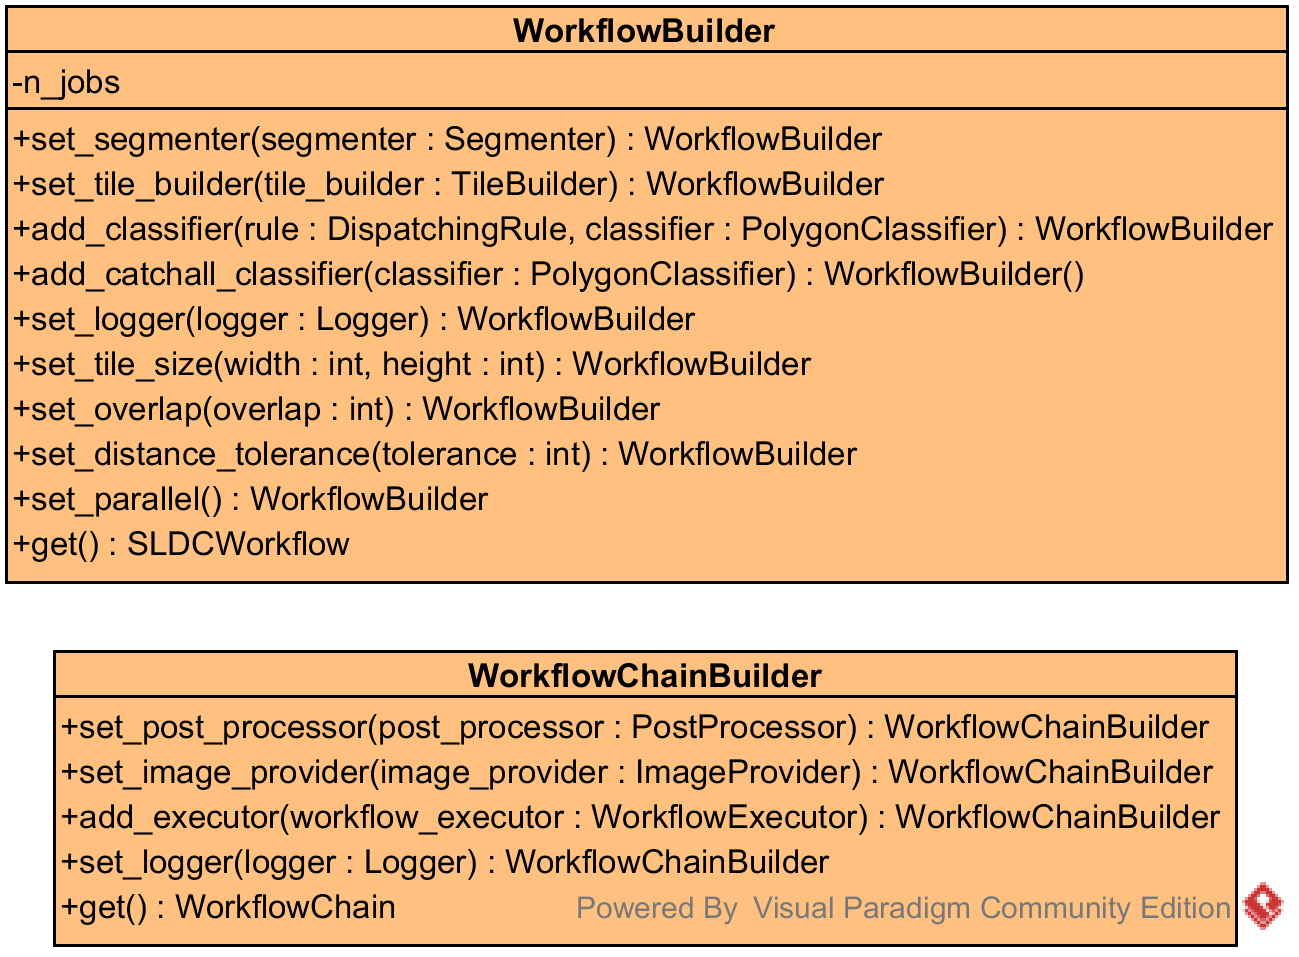
\includegraphics[scale=0.75]{image/uml_builder.png}
	\caption{Package \texttt{sldc.builder}.}
	\label{fig:uml_builder}
\end{figure}
 
\subsubsection{Parallelization}
\label{sssec:work_parallel}
As stated in the requirements, the framework should allow the user to take advantage of parallelism to reduce overall execution time. First, it is important to understand few things about parallelism in Python. The language natively provides packages for parallelizing code: \texttt{multiprocessing} and \texttt{threading}. A library called \texttt{joblib} was built on top of those packages and provides a high level interface for writing parallelized loops in a very concise way.  As far as threading is concerned, some implementation of the interpreter (i.e. CPython) prevents the threads to execute concurrently because of the Global Interpreter Lock (GIL). This lock is acquired by the thread which executes and prevents the other threads to access the interpreter for executing their own code. Therefore, it is advised in the language documentation to use multiprocessing to ensure that code is effectively executed in parallel whatever the interpreter implementation. Working over several processes however has the drawback of requiring inter-process communication. Particularly, the processes must be passed the data to treat and return the generated results to the main process. This is handled by \texttt{joblib} using serialization. Especially, the elements to be processed in parallel are queued. When a process becomes available, an element is dequeued, serialized and transferred to this process. When it terminates its execution, the results are themselves serialized and returned to the main process. This organization has the drawback of triggering as many serialization and deserialization as there are objects to process. Yet, such operations induce a non-negligible overhead that can be overcome by passing batches of elements instead of single elements to the processes. Another important point is the fact that \texttt{multiprocessing} doesn't support nested parallel loops. This constraint imposes therefore at most one level of parallelism. That is, a code executing in a spawned process cannot itself spawn other processes. All these language and library specific constraints were taken into account when including the parallelism to the framework.

How the parallelism will be implemented is now known, the question yet to be answered is where it will be applied. Several steps of the algorithm can be retained as candidates because of their highly parallelizable nature. In this case, highly parallelizable means that the parallelization can be done without any synchronization mechanisms except the ones provided by \texttt{joblib}. Typically, this is the case for operations which imply several independent computations. At the workflow level, the candidates steps are tiles segmentation and location, polygons dispatching and polygons classification. At the chaining level, the processing of the images generated by the \texttt{ImageProvider} is another candidate. 

Whereas applying parallelism at the chaining level is very easy, the idea was abandoned for the following reasons: it would prevent the parallelization at the workflow level (because of the nested parallel loops issue) and it can be done manually by the implementer. Indeed, he just has to launch its program one time on each image to obtain the same result.  

At the workflow level, both dispatching and classification parallelization were dropped because it would require more work and the need was less obvious than for segmentation and location. Indeed, it was assumed that the segmentation procedure provided by the implementer was likely to be computationally expensive. So the advantage resulting from this parallelization might be greater than for the two other operations. 

The parallelization itself is handled in the \texttt{SLDCWorkflow} class. In order to reuse the same pool of processes for every call of the \texttt{execute} method, this pool must be passed to the constructor of the workflow object as a \texttt{joblib.Parallel} object. In order to provide more feedback about progress to the user in the sequential case, two implementations of segmentation and location were made. Therefore, the workflow switches to one or another implementation according to the number of jobs specified by the user. The parallel implementation first splits the tiles in batches and then submits them to the various processes using the pool. After that, it aggregates the returned data. Especially, in addition to the found polygons, each process returns a \texttt{WorkflowTiming} object containing the loading, segmentation and location times it recorded when processing its assigned tiles. Those objects are merged with the \texttt{WorkflowTiming} to be returned by the \texttt{execute} method.

To avoid any concurrency problems, all classes of the framework were developed to be thread safe. This was done by making those classes immutable whenever possible or by avoiding to use shared resource. The only classes which couldn't verify this rule are \texttt{WorkflowTiming}, \texttt{StandardOutputLogger} and \texttt{FileLogger}. The timing objects can indeed be updated with new time recordings after their creation. The loggers by printing log messages access shared resources (e.g. standard output, files,...). To prevent any problem, the \texttt{Logger} was added a lock object to synchronize the call to the \texttt{\_print} abstract method which actually implements the submission of the message to the resource.

\subsection{Testing}
\label{ssec:work_test}
In order to ensure that the various components of the framework are working as expected in some predefined conditions and to prevent those components to be broken by further refactoring, some tests were written using the \texttt{unittest} package of Python. Those tests can also be found on GitHub in the folder \texttt{tests}. 

The tests were focused on components containing actual logic, that is, the classes \texttt{Locator}, \texttt{DispatcherClassifier}, \texttt{Merger} and \texttt{TileTopology}. The workflow construction and execution was also tested on two use cases. The first is presented in Section \ref{ssec:work_toy_example} and the second consists in finding a big white circle in a image with black background. Finally, there are fifteen tests and they yield a code coverage of 72 \%.\\

\subsection{Toy example}
\label{ssec:work_toy_example}
Now that the implementation was presented and detailed, this section aims at highlighting how easy it is to apply the framework to solve a problem. The problem in question is very simple and consists in finding grey and white squares and circles within a greyscale image with a black background (see in Figure \ref{fig:toy_example}). In addition to locate the shapes, the algorithm should return the information about whether a shape is a circle or a square and also return a label indicating its color (grey or white). 

To apply the workflow philosophy, the implementer should first encapsulate its image custom format in a class extending \texttt{Image}. For this example, a simple NumPy array can be used to represent the image. The definition of the image class is given in Listing \ref{lst:toy_image}. The next component to be defined is the segmentation algorithm that will actually detects the objects. In this case, this algorithm can be implemented using a simple thresholding (every pixel of which the value is greater than 0 belongs to an object). This logic should be defined in a class implementing the \texttt{Segmenter} interface. The definition of this class is shown in Listing \ref{lst:toy_segment}. Thanks to the usage of NumPy arrays, the implementation of the segmentation is really concise. 

The next step is the definition of the dispatching rules that will redirect the objects to an appropriate classifier. Especially, the idea is to take advantage of dispatching for detecting whether a shape is a circle or a square. In this case, two rules are needed: one that evaluates to true the circle polygons and another one which evaluates to true square polygons. One way to distinguish circles and squares is using the circularity shape factor. It is a real value between 0 and 1 which measures how close the shape of an object is to that of a circle. Especially, perfect circles have a circularity 1 and straight lines have a circularity 0. In this case, because the shape is discretized in the image, the algorithm will never produce perfect circles so detecting circular shapes must be done by thresholding the circularity. Particularly, polygons having a circularity greater than 0.85 can be considered circles while the others can be considered squares. The implementation of the dispatching rules are given in Listing \ref{lst:toy_rules}. Thanks to the Python list comprehension syntax, the definition of the rules is again really concise. 

Now that the segmentation and dispatching rules are defined, the last missing element is the classifier. In this case, it should produce the last desired information which is the color of the shapes. A simple idea is to use the polygon to retrieve the central pixel of the shape. Then, the greyscale value of this pixel can be checked to identify whether the color of the shape is white or grey. The implementation of the classifier is given in Listing \ref{lst:toy_classify}. In the context of this example, the image to be processed might not be large. However, the classifier is implemented so that the full image is never loaded into memory. Indeed, before extracting the pixels, the window boxing the polygon is extracted from the image and only the NumPy representation of this window is loaded into memory (see \texttt{image.window\_from\_polygon()} and \texttt{window.np\_image} method calls). 

\begin{figure}
	\center
	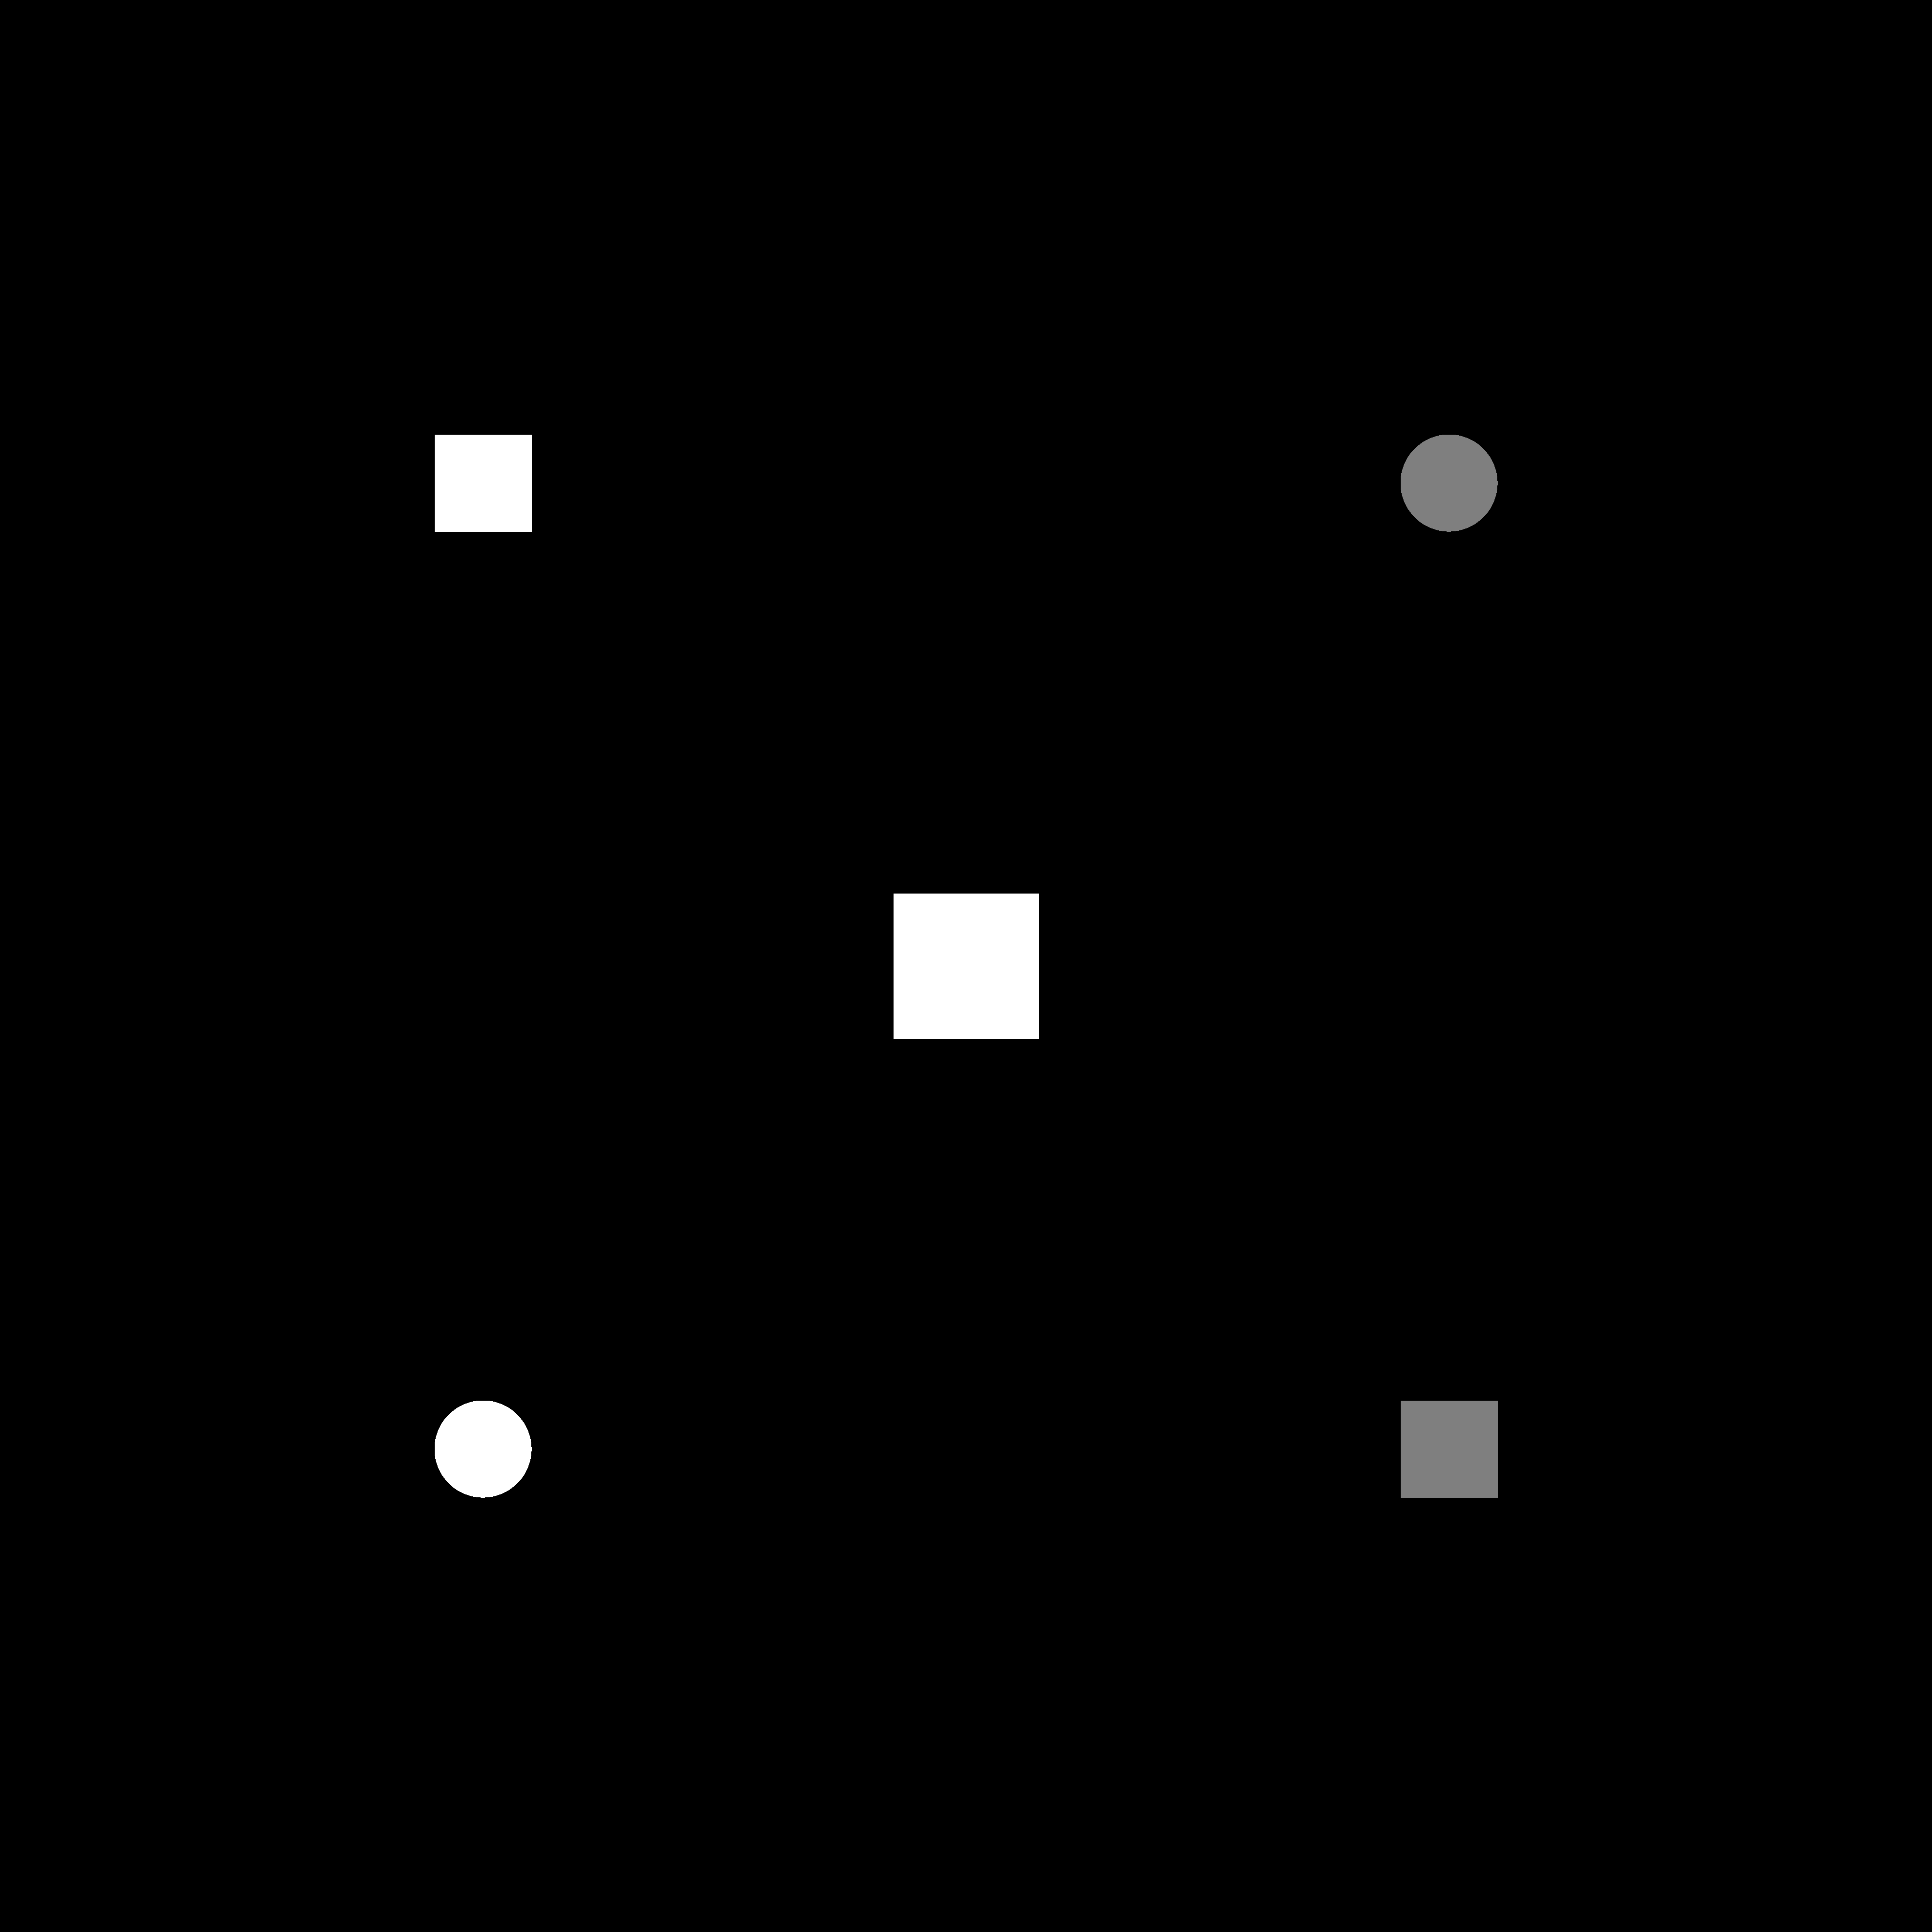
\includegraphics[scale=0.05]{image/toy_example.png}
	\caption{Example image to be processed for the toy example}
	\label{fig:toy_example}
\end{figure}

\begin{python}[label={lst:toy_image},caption={Toy example - Encapsulating custom image format}] 
class NumpyImage(Image):
    """An image represented as a NumPy ndarray"""
    def __init__(self, np_image):
        self._np_image = np_image

    @property
    def np_image(self):
        return self._np_image

    @property
    def channels(self):
        shape = self._np_image.shape
        return shape[2] if len(shape) == 3 else 1

    @property
    def width(self):
        return self._np_image.shape[1]

    @property
    def height(self):
        return self._np_image.shape[0]
\end{python}

\begin{python}[language=python,label={lst:toy_rules},caption={Toy example - Dispatching rules}] 
class CircleRule(DispatchingRule):
    """Dispatching rule which matches circles"""
    def evaluate_batch(self, image, polygons):
        return [circularity(polygon) > 0.85 for polygon in polygons]
        
class SquareRule(DispatchingRule):
    """Dispatching rule which matches squares"""
    def evaluate_batch(self, image, polygons):
        return [circularity(polygon) <= 0.85 for polygon in polygons]
\end{python}

\begin{python}[language=python,label={lst:toy_classify},caption={Toy example - Classifier}] 
class ColorClassifier(PolygonClassifier):
    """Classifier that predicts the color of a shape"""
    GREY = 0
    WHITE = 1
    def predict_batch(self, image, polygons):
        classes = []
        for polygon in polygons:
            # Fetch center pixel
            window = image.window_from_polygon(polygon)
            sub_image = window.np_image
            c_x = int(polygon.centroid.x) - window.offset_x
            c_y = int(polygon.centroid.y) - window.offset_y
            pxl = sub_image[c_y][c_x]
            # Generate the label based on the pixel color
            if pxl == 255:
                classes.append(self.WHITE)
            elif 0 < pxl < 255:
                classes.append(self.GREY)
            else:
                classes.append(None)
        return classes, [1.0] * len(polygons)

\end{python}

\begin{python}[language=python,label={lst:toy_segment},caption={Toy example - Segmentation implementation}] 
class CustomSegementer(Segmenter):
    """Every non black pixel are in an object of interests"""
    def segment(self, image):
        return (image > 0).astype("uint8")
\end{python}

\begin{python}[language=python,label={lst:toy_build_and_call},caption={Toy example - Applying the framework}] 
# Build the workflow
builder = WorkflowBuilder(n_jobs=1)
builder.set_segmenter(CustomSegmenter())
builder.add_classifier(CircleRule(), ColorClassifier())
builder.add_classifier(SquareRule(), ColorClassifier())
workflow = builder.get()

# Execute
results = workflow.process(NumpyImage(image))
\end{python}

\section{Improvements and future works}
\label{sec:work_future_works}
This section presents some possible improvements that could be performed to increase the ease of use and the performances of the framework. 

\subsection{Memory management}
Under the hood, Python wraps everything into objects \cite{pythonleaks2016}. This includes primitive types such as integers. Moreover, as memory allocation is an expensive operation, those objects are pooled by the Python runtime. Especially, it stores list of free objects which can be re-used when the user implicitly request them. The problem is that the free objects in those lists are never released and therefore, from the operating system point of view, the memory needed by the program only increases. It might worth checking the impact of this memory management policy over the memory consumption of the framework. Especially, it if happens to be a problem, the framework should be analyzed to check which parts yield a high memory consumption and those parts should be re-written.

\subsection{Location algorithm}
The location algorithm sometimes fails at generating polygons for all the detected objects in the segmentation mask. This happens when some objects' masks are ill-formed yielding invalid polygon containing self-intersections. A self-intersection is a point where two edges of a polygon intersect or are colinear. A first procedure for cleaning the segmentation mask has been implemented but it seems not be sufficient to prevent invalid polygons to be generated. An improvement would therefore consists in understanding which kind of patterns yield self-intersections and to implement a procedure for cleaning those patterns. 

\subsection{Parallelization}
Parallelization was successfully applied for tiles segmentation and location but other phases of the workflow might also benefit from it. For instance, when the dispatching and classification procedures cannot be parallelized by the implementer, those steps are executed sequentially no matter what. This can present a major issue especially when the number of objects found in the image is high. A possible improvement would consist in splitting the detected objects in batches and to execute dispatching and classification for each batch on different processes. 

Another critical point is the workflow executor. Indeed, when the implementer implements a processing chain, the first executor typically processes the full image and the parallelization can happen at the workflow level. According to the number of objects detected by this first step, the subsequent executors might generate a lot of image windows to be processed by other workflows. Currently, all those windows must be processed sequentially which can potentially yield huge execution times. An improvement would then consist in parallelizing those windows processing. This would have to be implemented carefully as this parallelization shouldn't clash with the one implemented at the workflow level (see Section \ref{sssec:work_parallel} for the nested parallel loops issue).

Finally, it would be interesting to optimize the parallelization of the tiles processing. Currently, batches of tile objects are passed to the processes which requires a potentially heavy serialization. Indeed, tiles being defined by the implementer, he could stores heavy objects in the class attributes. A possible improvement would therefore consist in passing batches of tiles identifiers instead of the tile themselves and to use the tile topology to re-build the tiles on each process. 

\label{sec:work_improvements}